%%%%%%%%%%%%%%%%%%%%%%%%%%%%%%%%%%%%%%%%%
% Masters/Doctoral Thesis 
% LaTeX Template
% Version 2.4 (22/11/16)
%
% This template has been downloaded from:
% http://www.LaTeXTemplates.com
%
% Version 2.x major modifications by:
% Vel (vel@latextemplates.com)
%
% This template is based on a template by:
% Steve Gunn (http://users.ecs.soton.ac.uk/srg/softwaretools/document/templates/)
% Sunil Patel (http://www.sunilpatel.co.uk/thesis-template/)
%
% Template license:
% CC BY-NC-SA 3.0 (http://creativecommons.org/licenses/by-nc-sa/3.0/)
%
%%%%%%%%%%%%%%%%%%%%%%%%%%%%%%%%%%%%%%%%%

%----------------------------------------------------------------------------------------
%	PACKAGES AND OTHER DOCUMENT CONFIGURATIONS
%----------------------------------------------------------------------------------------

\documentclass[
11pt, % The default document font size, options: 10pt, 11pt, 12pt
%oneside, % Two side (alternating margins) for binding by default, uncomment to switch to one side
ngerman, % english, % ngerman for German
singlespacing, % Single line spacing, alternatives: onehalfspacing or doublespacing
%draft, % Uncomment to enable draft mode (no pictures, no links, overfull hboxes indicated)
%nolistspacing, % If the document is onehalfspacing or doublespacing, uncomment this to set spacing in lists to single
%liststotoc, % Uncomment to add the list of figures/tables/etc to the table of contents
%toctotoc, % Uncomment to add the main table of contents to the table of contents
%parskip, % Uncomment to add space between paragraphs
%nohyperref, % Uncomment to not load the hyperref package
headsepline, % Uncomment to get a line under the header
%chapterinoneline, % Uncomment to place the chapter title next to the number on one line
%consistentlayout, % Uncomment to change the layout of the declaration, abstract and acknowledgements pages to match the default layout
]{MastersDoctoralThesis} % The class file specifying the document structure

\usepackage[utf8]{inputenc} % Required for inputting international characters
\usepackage[T1]{fontenc} % Output font encoding for international characters
\usepackage{todonotes} % Hints for TO-DOs in text (also missing figures,...)
\usepackage{palatino} % Use the Palatino font by default
\PassOptionsToPackage{hyphens}{url}\usepackage{hyperref}
\usepackage{amsmath,amssymb,amsthm}
\usepackage{mathtools}
\usepackage{hhline}  % For double lines without interupt in tabular environment

\usepackage{tikz} % For generating diagrams, plotting tensors,...
\usetikzlibrary{matrix,calc}

\usepackage{algorithm} % basic pseudocode package
\usepackage{algorithmicx} % For pseudocode, algorithm environment
\usepackage{algpseudocode} % defines stuff like\Procedure for algorithmicx
\algtext*{EndWhile}% Remove "end while" text
\algtext*{EndIf}% Remove "end if" text
\algtext*{EndFor}% Remove "end for" text
\algtext*{EndProcedure}% Remove "end procedure" text
\algtext*{EndFunction}% Remove "end function" text
\algnewcommand{\LineComment}[1]{\State \(\triangleright\) #1} %For line comments

\makeatletter 
 \renewcommand{\ALG@name}{Algorithmus} %change "Algorithm" to "Algorithmus"
\makeatother  
\renewcommand{\listalgorithmname}{Liste der Pseudocodes}

  
% biber and biblatex need to be compatibile (see "Compatibility matrix").. which is kinda strange and needs maybe manual installation of one of the packages
\usepackage[backend=biber,style=numeric,natbib=true]{biblatex} 

\addbibresource{lit.bib} % The filename of the bibliography

\usepackage[autostyle=true]{csquotes} % Required to generate language-dependent quotes in the bibliography

%----------------------------------------------------------------------------------------
%	MARGIN SETTINGS
%----------------------------------------------------------------------------------------

\geometry{
	paper=a4paper, % Change to letterpaper for US letter
	inner=2.5cm, % Inner margin
	outer=3.8cm, % Outer margin
	bindingoffset=.5cm, % Binding offset
	top=1.5cm, % Top margin
	bottom=1.5cm, % Bottom margin
	%showframe, % Uncomment to show how the type block is set on the page
}

%----------------------------------------------------------------------------------------
%	THESIS INFORMATION
%----------------------------------------------------------------------------------------

\thesistitle{Uncertainty Quantification für die Klein-Gordon-Gleichung} % Your thesis title, this is used in the title and abstract, print it elsewhere with \ttitle
\supervisor{Prof. Dr. Tobias \textsc{Jahnke}} % Your supervisor's name, this is used in the title page, print it elsewhere with \supname
\examiner{} % Your examiner's name, this is not currently used anywhere in the template, print it elsewhere with \examname
\degree{Master of Science} % Your degree name, this is used in the title page and abstract, print it elsewhere with \degreename
\author{Daniel \textsc{Dittmar}} % Your name, this is used in the title page and abstract, print it elsewhere with \authorname
\addresses{} % Your address, this is not currently used anywhere in the template, print it elsewhere with \addressname

\subject{Numerische Mathematik} % Your subject area, this is not currently used anywhere in the template, print it elsewhere with \subjectname
\keywords{Klein-Gordon-Gleichung, Zeitintegration, Splitting, Uncertainty quantification, General Polynomial Chaos} % Keywords for your thesis, this is not currently used anywhere in the template, print it elsewhere with \keywordnames
\university{\href{http://www.kit.edu}{Karlsruher Institut für Technologie}} % Your university's name and URL, this is used in the title page and abstract, print it elsewhere with \univname
\department{\href{http://www.math.kit.edu/ianm}{Institut für Angewandte und Numerische Mathematik}} % Your department's name and URL, this is used in the title page and abstract, print it elsewhere with \deptname
\group{\href{http://www.math.kit.edu/ianm3}{Arbeitsgruppe Wissenschaftliches Rechnen}} % Your research group's name and URL, this is used in the title page, print it elsewhere with \groupname
\faculty{\href{http://www.math.kit.edu/ianm3}{Fakultät für Mathematik}} % Your faculty's name and URL, this is used in the title page and abstract, print it elsewhere with \facname

\AtBeginDocument{
\hypersetup{pdftitle=\ttitle} % Set the PDF's title to your title
\hypersetup{pdfauthor=\authorname} % Set the PDF's author to your name
\hypersetup{pdfkeywords=\keywordnames} % Set the PDF's keywords to your keywords
\hypersetup{colorlinks=false} % Links in pdf but not in printed
}

\include{defs}

\begin{document}

\frontmatter % Use roman page numbering style (i, ii, iii, iv...) for the pre-content pages

\pagestyle{plain} % Default to the plain heading style until the thesis style is called for the body content

%----------------------------------------------------------------------------------------
%	TITLE PAGE
%----------------------------------------------------------------------------------------

\begin{titlepage}
\begin{center}

\includegraphics{Figures/kitlogo_de_rgb.pdf} % University/department logo - uncomment to place it
\linebreak
\vspace*{.06\textheight}
{\scshape\LARGE \univname\par}\vspace{1.5cm} % University name
\textsc{\Large Masterarbeit}\\[0.5cm] % Thesis type

\HRule \\[0.4cm] % Horizontal line
{\huge \bfseries \ttitle\par}\vspace{0.4cm} % Thesis title
\HRule \\[1.5cm] % Horizontal line
 
\begin{minipage}[t]{0.4\textwidth}
\begin{flushleft} \large
\emph{Autor:}\\
{\authorname} % Author name - remove the \href bracket to remove the link
\end{flushleft}
\end{minipage}
\begin{minipage}[t]{0.4\textwidth}
\begin{flushright} \large
\emph{Betreuer:} \\
\href{http://www.math.kit.edu/ianm3/~jahnke}{\supname} % Supervisor name - remove the \href bracket to remove the link  
\end{flushright}
\end{minipage}\\[3cm]
 
\vfill


\groupname\\\deptname\\[2cm] % Research group name and department name
 
\vfill

{\large \today}\\[4cm] % Date

 
\vfill
\end{center}
\end{titlepage}

%----------------------------------------------------------------------------------------
%	DECLARATION PAGE
%----------------------------------------------------------------------------------------

\begin{declaration}
\addchaptertocentry{\authorshipname} % Add the declaration to the table of contents
\noindent Ich, Daniel Dittmar, versichere wahrheitsgemäß, die Arbeit selbstständig verfasst, alle benutzten Quellen und Hilfsmittel vollständig und genau angegeben und alles kenntlich gemacht zu haben, was aus Arbeiten anderer unverändert oder mit Abänderungen entnommen wurde sowie die Satzung des KIT zur Sicherung guter wissenschaftlicher Praxis in der jeweils gültigen Fassung beachtet zu haben.
 \\[0.5cm]
\noindent Unterschrift:\\
\rule[0.5em]{25em}{0.5pt} % This prints a line for the signature
 
\noindent Datum:\\
\rule[0.5em]{25em}{0.5pt} % This prints a line to write the date
\end{declaration}

\cleardoublepage

%----------------------------------------------------------------------------------------
%	QUOTATION PAGE
%----------------------------------------------------------------------------------------
%
%\vspace*{0.2\textheight}
%
%\noindent\enquote{\itshape If you can't explain something to a first year student, then %you haven't really understood it.}\bigbreak
%
%\hfill Richard Feynman, et al.
%
%----------------------------------------------------------------------------------------
%	ABSTRACT PAGE
%----------------------------------------------------------------------------------------

\begin{abstract}
\addchaptertocentry{\abstractname} % Add the abstract to the table of contents
Die \it{uncertainty quantification} ermöglicht es, partielle Differentialgleichungen aus einem stochastischen Blickwinkel zu betrachten. Dies ermöglicht es solche Parameter der Gleichung, die auf schwankenden Messwerten oder intrinsischem Zufall basieren, direkt im Modell ohne weitere Vereinfachung zu verankern.\\
Diese Arbeit untersucht am Beispiel einer verallgemeinerten linearen Klein-Gordon-Gleichung den Einfluss von stochastischen Parametern auf Erwartungswert und Varianz der zufallsabhängigen Lösung. Dabei werden verschiedene Lösungsansätze und Beispiele auf Implementierungsebene miteinander verglichen. Das Ziel ist es, Stärken und Schwächen der Ansätze besser zu verstehen und Einblicke in die Wahl von Hyperparametern, wie beispielsweise dem benötigten Polynomgrad, zu bekommen. Ein weiterer Fokus liegt auf der Praktikabilität der Methoden für mehrdimensionale Zufallsvariablen; der Einfachheit halber werden sich gezeigte Beispiele aber auf eine räumliche Dimension beschränken.
\end{abstract}

%----------------------------------------------------------------------------------------
%	ACKNOWLEDGEMENTS
%----------------------------------------------------------------------------------------

\begin{acknowledgements}
\addchaptertocentry{\acknowledgementname} % Add the acknowledgements to the table of contents
Hiermit danke ich allen, die mir während meines Studiums hilfreich zur Seite standen und mich immer unterstützt haben. Im Speziellen danke ich meine Eltern, Großeltern und meinem Bruder Fabian für ihre uneingeschränkte Unterstützung.\\ 
Für die Unterstützung bei meiner Masterarbeit und für hilfreiche Ratschläge danke ich insbesondere meinem Betreuer Herrn Jahnke.\\
Ein großes Dankeschön geht an Verena Volkmer für ihr konstruktives Korrekturlesen und ihre vielen Verbesserungsvorschläge.
\end{acknowledgements}

%----------------------------------------------------------------------------------------
%	LIST OF CONTENTS/FIGURES/TABLES PAGES
%----------------------------------------------------------------------------------------

\tableofcontents % Prints the main table of contents

%\listoffigures % Prints the list of figures

%\listoftables % Prints the list of tables

%----------------------------------------------------------------------------------------
%	ABBREVIATIONS
%----------------------------------------------------------------------------------------

\begin{abbreviations}{ll} % Include a list of abbreviations (a table of two columns)

\textbf{KGG} & \textbf{K}lein-\textbf{G}ordon-\textbf{G}leichung\\
\textbf{sKGG} & \textbf{s}tochastische \textbf{K}lein-\textbf{G}ordon-\textbf{G}leichung\\
\textbf{FFT} & \textbf{F}ast-\textbf{F}ourier-\textbf{T}ransformation\\
\textbf{gPC} & \textbf{g}eneral \textbf{P}olynomial-\textbf{C}haos\\
\textbf{MC} & \textbf{M}onte-\textbf{C}arlo\\
\textbf{QMC} & \textbf{Q}uasi-\textbf{M}onte-\textbf{C}arlo\\
\textbf{LGS} & \textbf{L}ineares \textbf{G}leichungs\textbf{s}ystem\\
\textbf{MI} & \textbf{M}atrix-\textbf{I}nvertierung (Collocation durch Interpolation)\\
\textbf{DP} & \textbf{D}iskrete \textbf{P}rojektion (Collocation durch diskrete Projektion)\\


\end{abbreviations}

%----------------------------------------------------------------------------------------
%	SYMBOLS
%----------------------------------------------------------------------------------------

\begin{symbols}{lll} % Include a list of Symbols (a three column table)
$t$ & Zeit & Einheitslose nicht-negative reelle Variable\\
$x$ & Ort & Einheitslose (mehrdimensionale) reelle Ortsvariable\\
$\dt{u}$ & Ableitung nach t & Für differenzierbares $u\colon\R\to \R$\\ 
$\Laplace$ & Laplace& Laplace Operator im Ort $\Laplace u(x_1,x_2)=\frac{\text{d}^2}{\text{d}x^2_1}u(x_1,x_2)+\frac{\text{2}^2}{\text{d}x^2_d}u(x_1,x_2)$ \\
$\Torus$ & eindimensionaler Torus & $\Torus=\R/(2\pi\Z)$\\
$\tau$ & Zeitschrittweite & $0<\tau<1$\\
$d$ & räumliche Dimension & $d\in\N$\\
$\mathcal{O}$ & Landau-Symbol & Asymptotischer Aufwand/Verhalten\\

%Symbol & Name & Description \\

\end{symbols}


%----------------------------------------------------------------------------------------
%	THESIS CONTENT - CHAPTERS
%----------------------------------------------------------------------------------------

\mainmatter % Begin numeric (1,2,3...) page numbering

\pagestyle{thesis} % Return the page headers back to the "thesis" style

% Include the chapters of the thesis as separate files from the Chapters folder
% Uncomment the lines as you write the chapters

% Chapter 1

\chapter{Einführung} % Main chapter title

\label{Chapter1} % For referencing the chapter elsewhere, use \ref{Chapter1} 

% Chapter 2

\chapter{Stochastische Hintergründe}
In diesem Kapitel werden wir erläutern, wie man stochastische Einflüsse auf die KGG darstellen kann. Anschließend werden wir mit der Monte-Carlo Methode bereits ein erstes Verfahren kennen lernen, um den Erwartungswert und die Varianz der zufallsabhängigen Lösung der KGG zu bestimmen.


\section{Grundbegriffe}
Wir geben keine Einführung in die klassische Wahrscheinlichkeitstheorie, werden aber die relevanten Begriffe und Definitionen an dieser Stelle kurz wiederholen. Es sei angemerkt, dass neben den vorgestellten stetigen Verteilungen auch diskrete Verteilungen wie die Poisson-Verteilung existieren und sich durch die selbe Theorie beschreiben lassen. Um die Notation zu vereinfachen, werden wir jedoch ausschließlich stetige Verteilungen betrachten.

\begin{mathdef}[Wahrscheinlichkeitsraum]
Ein Wahrscheinlichkeitsraum $(\Omega,\mathcal{F},P)$ ist ein Tripel bestehend aus 
\begin{itemize}
\item der abzählbaren nichtleeren Ergebnismenge $\Omega$
\item der $\sigma$-Algebra der Ereignisse $\mathcal{F}$ über der Grundmenge $\Omega$
\item dem Wahrscheinlichkeitsmaß $P\colon\mathcal{F}\to [0,1]$
\end{itemize}
\end{mathdef}

\begin{mathdef}[Verteilungsfunktion]
Die Verteilungsfunktion $F_Y$ der Zufallsvariablen $Y\colon\Omega\to\R$ ist definiert durch
\[F_Y(y)\coloneqq P(Y\le y)=P(\left\lbrace \omega\in\Omega |\: Y(\omega)\le y\right\rbrace),\quad y\in\R\]
\end{mathdef}
\begin{mathdef}[Dichte einer Verteilung]
Existiert zu der Verteilungsfunktion $F_Y$ der Zufallsvariablen $Y\colon\R\to\R$ eine Funktion $\rho_Y\colon\R\to\R_{\ge 0}$ mit
\[F_Y(y)=\int_{-\infty}^y\rho_Y(z)dz,\quad y\in\R\]
so nennen wir diese die Dichte von $F_Y$.
\end{mathdef}
\begin{mathdef}[Stochastische Unabhängigkeit]
Ist $(\Omega,\mathcal{F},P)$ ein Wahrscheinlichkeitsraum und $Y_1, Y_2\colon \Omega\to\R$ zwei reelle Zufallsvariablen, so nennt man $Y_1$ und $Y_2$ (stochastisch) unabhängig, genau dann wenn
\[P(Y_1\in B_1,Y_2\in B_2)=P(Y_1\in B_1)P(Y_2\in B_2)\]
für alle $B_1,B_2\in \mathcal{B}(\R)$, der Borelschen $\sigma$-Algebra über $\R$.
\end{mathdef}
\begin{mathbsp}
Ist $\mathcal{N}(\mu, \sigma^2)$ die Normalverteilung mit Parametern $\mu\in\R$ und $\sigma^2>0$ so gilt für ihre Dichtefunktion
\[\rho_Y(y)=\frac{1}{\sqrt{2\pi\sigma^2}}e^{-\frac{(y-\mu)^2}{2\sigma^2}},\quad y\in\R\]
Ist $\mathcal{U}(a,b)$ die Gleichverteilung auf $(a,b)$ so gilt für ihre Dichtefunktion
\[\rho_Y(y)=\begin{cases}\frac{1}{b-a},\quad &y\in (a,b)\\ 0, \quad &\text{sonst} \end{cases}\]
\end{mathbsp}
Folgende Definitionen werden die später hauptsächlich untersuchten Eigenschaften von zufallsabhängigen Größen darstellen.
\begin{mathdef}[Erwartungswert und Varianz]
Ist $Y\colon\R\to\R$ eine reelle Zufallsvariable mit Dichte $\rho_Y$ so ist definieren wir den Erwartungswert von $Y$ als
\[\mu_Y=\E[Y]=\int_{-\infty}^\infty y\rho_Y(y)dy\]
und die Varianz von $Y$ als 
\[\mu_Y^2=\text{var}(Y)=\int_{-\infty}^\infty (y-\mu_Y)^2\rho_Y(y)dy\]
\end{mathdef}
Ohne Beweis präsentieren wir die Inversionsmethode. Diese ist nützlich, um aus Zufallsvariablen einer bestimmten Verteilung Zufallsvariablen einer anderen Verteilung zu gewinnen. In der Numerik ist dies ist essentiell für die Generation von Pseudozufallszahlen von beliebigen Verteilungen, aber auch für die "`stochastische Normierung"' von verschiedenen Zufallsvariablen zu einem gemeinsamen Wahrscheinlichkeitsraum, auf dem dann Erwartungswerte berechnet werden können.
\begin{maththeorem}[Inversionsmethode]
\label{thinversionsmethode}
Ist $Y$ eine reelle Zufallsvariable mit Verteilungsfunktion $F_Y$, so definieren wir deren Quantilfunktion als
\[F_Y^{-1}(p)\coloneqq \inf\lbrace y\in\R |\: F_Y(y)\ge p\rbrace,\quad p\in\R\]
Dann gilt
\begin{itemize}
\item $z\le F_Y(y)\iff F_Y^{-1}(z)\le y$\\
\item Falls $Z$ gleichverteilt in $(0,1)$ ist, dann hat $F_Y^{-1}(Z)$ die Verteilungsfunktion $F_Y$. 
\end{itemize}
\end{maththeorem}
Der auch Gesetz der großen Zahlen genannte Zentrale Grenzwertsatz sei ebenfalls genannt, da er die Grundlage für das erste Verfahren zur Berechnung von Erwartungswert und Varianz darstellt.
\begin{maththeorem}[Zentraler Grenzwertsatz]
\label{thzentralgrenzwert}
Seien $Y_1,Y_2,\dots,Y_n$ unabhängige und identisch verteilte Zufallsvariablen mit $\E[Y]_i=\mu$ und $\text{var}(Y_i)=\sigma^2<\infty$ Der Mittelwert sei definiert als
\[\overline{Y}\coloneqq \frac{1}{n}\sum_{i=1}^nY_i\]
und skaliert durch
\[Z_n=\sqrt{n}\left(\frac{\overline{Y}-\mu}{\sigma}\right)\]
Dann konvergiert für $n\to\infty$ die Verteilungsfunktion von $Z_n$ zu einer $\mathcal{N}(0,1)$ verteilten Verteilungsfunktion.
\end{maththeorem}
\begin{mathdef}[Zufallsvektoren]
Wir nennen $Y=(Y_1,\dots,Y_n)$ einen $n$-dimensionalen Zufallsvektor (häufig auch einfach $n$-dimensionale Zufallsvariable), wenn die Komponenten $Y_1,\dots,Y_n\colon\Omega\to\R$ eindimensionale Zufallsvariablen sind. Besitzt jede Komponente $Y_i$ eine Dichte $\rho_{Y_i}$, so ist die gemeinsame Dichte
\[\rho_Y=\prod_{i=1}^n \rho_{Y_i}\]
und die Verteilungsfunktion lässt sich darstellen als
\[F_Y(y_1,\dots,y_n)=\int_{-\infty}^{y_1}\dots\int_{-\infty}^{y_n}\rho_Y(z_1,\dots,z_n)dy_1\dots dy_n\]
\end{mathdef}
Weitere wichtige Begriffe, die aber in dieser Arbeit nicht in den Vordergrund rücken werden, seien stichwortartig genannt:
\begin{itemize}
\item Konvergenz $P$ fast sicher, Konvergenz in Wahrscheinlichkeit, Konvergenz in Verteilung\\
\item Bedingte Wahrscheinlichkeit, bedingte Erwartung
\item Unkorreliertheit vs. Unabhängigkeit
\item Momente höherer Ordnung, Moment-generierende Funktion
\end{itemize}

\section{Endliche Parametrisierung}
\label{secfiniteparam}
Dieser Abschnitt beschäftigt sich mit der Frage, wie man, ausgehend von einem potentiell unendlich dimensionalen Wahrscheinlichkeitsraum, eine endliche Charakterisierung desselben durch einen $n$-dimensionalen Zufallsvektor mit unabhängigen Komponenten erhalten kann. Die Bedingung der Unabhängigkeit ist dabei theoretisch zwar wenig einschränkend, aber eine sehr wichtige Grundlage für viele praktische numerische Verfahren.\\
Diese Frage tritt beispielsweise auf, wenn die Zufallsabhängigkeit im Modell nicht explizit über die Parameter einfließt, sondern ein zeitabhängiger stochastischer Prozess ist. Möglich wäre auch, dass die Zufallsabhängigkeit in endlich oder abzählbar vielen Modellparametern steckt, die einzelnen Parameter jedoch nicht stochastisch unabhängig sind.\\
Wir werden später stets davon ausgehen, dass bereits eine endliche Parametrisierung durch unabhängige Zufallsvariablen mit bekannter Verteilung vorliegt. Der Vollständigkeit aber seien hier kurz Methoden genannt, um das Parametrisierungsproblem zu lösen. Man beachte jedoch, dass einige der Methoden numerisch nicht umsetzbar oder ad-hoc Lösungen sind, die spezielle Annahmen benötigen. Dieser Abschnitt wurde aus \autocite[Kapitel 4.1+4.2]{dongbinxiu2010} übernommen, wo auch Visualisierungen und kleine Beispiele zu finden sind.

\subsection{Unabhängigkeit von endlich vielen Parametern}
Wenn die Zufallsabhängigkeit des Modells bereits durch endlich viele Modellparameter vorliegt, ist die Parameterisierung bereits gegeben. Wichtig ist dann, die unabhängigen Parameter zu identifizieren bzw. die Abhängigkeit zu konkretisieren.\\
Für normalverteilte Parameter ist dies auch auf einfache Weise möglich:
\begin{maththeorem}
\label{thgaussunabhg}
Sei $Y=(Y_1,\dots,Y_n)$ ein $\mathcal{N}(0,C)$ verteilter Zufallsvektor mit Kovarianzmatrix $C\in\R^{n\times n}$. Sei $Z\sim\mathcal{N}(0,I_n)$, wobei $I_n$ die n-dimensionale Einheitsmatrix ist, ein unkorrelierter Zufallsvektor. Für die Gaussverteilung ist Unkorreliertheit äquivalent zu Unabhängigkeit und die Komponenten von $Z$ sind somit unabhängig. Da $C$ reell und symmetrisch ist, existiert die Choleskyzerlegung $C=AA^T$ und es gilt
\[Y=AZ\sim\mathcal{N}(0,AA^T)=\mathcal{N}(0,C)\]
besitzt die gegebene Verteilung. Wir können folglich $Y$ durch stochastisch unabhängige Parameter $Z_1,\dots,Z_n$ darstellen.
\end{maththeorem}
Sind die Parameter nicht normalverteilt, so wird das Problem deutlich schwieriger und bis jetzt gibt es keine zufriedenstellende numerische Transformation, die entsprechendes zu Satz \ref{thgaussunabhg} leistet. Eine theoretische Möglichkeit bietet sich jedoch über die Rosenblatt Transformation, welche auf den in der Praxis selten bekannten bedingten Wahrscheinlichkeiten basiert.

\subsection{Parametrisierung von Zufallsprozessen}
Häufig sind die Zufallsabhängigkeiten des Modells nur durch Beobachtungen oder Messungen von Zufallsvariablen möglich. Wir schreiben diese als stochastischen Prozess $(Y_t,t\in T)$, wobei $T$ der Indexraum ist und $Y_t$ die beobachteten Zufallsvariablen. Wir suchen dann eine Transformation $R$, welche die Darstellung $Y_t=R(Z)$ mit Zufallsvektor $Z=(Z_1,\dots,Z_n)$ und unabhängigen Komponenten $Z_i$ erlaubt. Da $T$ potentiell ein unendlich dimensionaler Raum ist, kann diese Transformation nicht exakt sein und wir suchen nun eine in einem gewissen Sinne bestmögliche Approximation.\\
Die am häufigsten verwendete Technik ist dabei die Karhunen-Loeve Reihendarstellung.
\begin{mathdef}[Karhunen-Loeve Darstellung]
Sei $\mu_Y(t)$ der Erwartungswert des Prozesses $Y_t$ am Punkt $t$ und sei $C(t,s)=\text{cov}(Y_t,Y_s)$ die Kovarianzfunktion. Dann ist die Karhunen-Loeve Darstellung definiert als
\[Y_t(\omega)=\mu_Y(t)+\sum_{i=1}^\infty \sqrt{\lambda_i}\Psi_i(t)Z_i(\omega)\] wobei $\Psi_i$ die orthogonalen Eigenfunktionen und $\lambda_i$ die zugehörigen Eigenwerte des Eigenwertproblems
\[\int_T C(t,s)\Psi_i(s)ds=\lambda_i\Psi_i(t),\quad t\in T\]
sind. Die paarweise unkorrelierten Zufallsvariablen $Z_i(\omega)$ erfüllen
\[\E[Z_i]=0,\quad \E[Z_iZ_j]=\delta_{ij}\]
und sind definiert durch
\[Z_i(\omega)=\frac{1}{\sqrt{\lambda_i}}\int_T (Y_t(\omega)-\mu_Y(t))\Psi_i(t)dt\]
Um eine endliche Approximation zu erhalten wird die Reihe bei einem gewissen Index $n\in\N$ abgebrochen.
\end{mathdef}
Wiederrum erhält man daraus für normalverteilte Prozesse eine endliche Menge von unabhängigen Zufallsvariablen. Für nicht-normalverteilte Prozesse wird häufig dennoch die Karhunen-Loeve Darstellung verwendet und zusätzlich angenommen, dass die $Z_i$ unabhängig sind. Diese Vorgehensweise ist noch nicht zufrieden stellend und ein offenes Forschungsproblem.

\section{Formulierung der stochastischen KGG}
In Analogie zur Klein-Gordon-Gleichung (\ref{kgg}) definieren wir für einen Wahrscheinlichkeitsraum $(\Omega,\mathcal{F},P)$ und $Y\colon\Omega\to\R^N$ die stochastische Klein-Gordon-Gleichung (sKGG) für $y=Y(\omega)$ durch
\begin{align}
\label{skgg}
\dtt{u}(t,x,y)&=\alpha(y) \Laplace_x u(t,x,y) - \beta(x,\omega)u(t,x,y), \: t>0, \, x\in \Torus^d\\
u(0,x,y)&=u_0(x,y), \: x\in \Torus^d\\
\dt{u}(0,x,y)&=v_0(x,y), \: x\in \Torus^d
\end{align}
Die Lösung \[u(t,x,y)\colon [0,T]\times\Torus^d\times \R^N\to\R\] ist also eine zufallsabhängige Größe.\\
Dabei ist die grundlegende Annahme, dass (\ref{skgg}) $P$-fast-sicher wohl gestellt ist, d.h. die Menge an Punkten $\omega$ für welche die partielle Differentialgleichung mit fixem $y=Y(\omega)$ keine eindeutige Lösung besitzt ist eine Nullmenge bezüglich des Wahrscheinlichkeitmaßes $P$.\\
Ab sofort werden wir --wie in Kapitel \ref{secfiniteparam} diskutiert-- stets annehmen, dass die Komponenten $Y_i$ von $Y$ stochastisch unabhängige Zufallsvariablen mit bekannter Verteilung sind.
\begin{mathbsp}
\label{bsp:trial1}
Sei $Y=(Y_1)$ eine eindimensionale und in $(2,3)$ gleichverteilte Zufallsvariable. Dann gilt für $t>0$, $d\in\N$, $x=(x_1,\dots$, $x_d)\in\Torus^d$, $\hat{x}\coloneqq \sum_{i=1}^d x_i$ und $y=Y(\omega)$
\begin{align*}
u(t,x,y)&=2\cos(ty)\sin(\hat{x})\\
u_0(x,y)&=2\sin(\hat{x})\\
v_0(x,y)&\equiv 0
\end{align*}
löst die stochastische KGG (\ref{skgg}) für $\alpha(y)=\frac{y}{d}$ und $\beta(x,y)=y^2-y$\\
Für den Erwartungswert und Varianz von $u$ gelten
\begin{align*}
\E[u(t,x,Y)]&=\int_2^3u(t,x,y)dy=\frac{2}{t}\sin(\hat{x})(\sin(3t) - \sin(2t))\\
\text{var}(u(t,x,Y))&=\frac{1}{t}\sin^2(\hat{x})\left(2t + \sin(6t) - \sin(4t)\right)- \left(\frac{2}{t}\sin(\hat{x})(\sin(3t) - \sin(2t))\right)^2
\end{align*}
Um einen potentiellen Denkfehler zu vermeiden, weisen wir an dieser Stelle explizit darauf hin, dass 
\[\E[u(t,x,Y)]=\frac{2}{t}\sin(\hat{x})(\sin(3t) - \sin(2t))\neq 2\sin(\hat{x})\cos(\frac{5}{2}t)=u(t,x,\E[Y])\]
Dies erkennt man beispielsweise am Zeitpunkt $t=\frac{\pi}{2}$, wo gilt
\[\E[u(t,x,Y)]=-\sin(\hat{x})\pi \neq -\sin(\hat{x})\sqrt{2}=u(t,x,\E[Y])\]
Der Erwartungswert ist linear, die Abhängigkeiten von $y$ sind es aber nicht. Diese erste fehlgeschlagene Idee den Erwartungswert durch das Lösen eines deterministischen Systems zu erhalten, ist jedoch nicht vollends vergebens. Wir werden am Beispiel der Monte-Carlo-Methode sehen, dass wir dazu allerdings weit mehr als ein System lösen müssen.
\end{mathbsp}
Wir geben ein weiteres Referenzbeispiel an, wo nun auch die Ortsabhängigkeit von $\beta$ benutzt wird und auch ein Anfangswert abhängig von der Zufallsvariablen ist.
\begin{mathbsp}
Sei $Y=(Y_1)$ eine eindimensionale und in $(10,50)$ gleichverteilte Zufallsvariable. Dann gilt für $t>0$, $d=1$, $x\in\Torus$ und $y=Y(\omega)$
\begin{align*}
u(t,x,y)&=\frac{\cos(t)}{\sin(x) + y}\\
u_0(x,y)&=\frac{1}{\sin(x) + y}\\
v_0(x,y)&\equiv 0
\end{align*}
löst die stochastische KGG (\ref{skgg}) für \[\alpha(y)=y-2\text{  und  }\beta(x,y)=1 + (y-2)\left(\frac{\sin(x)}{\sin(x) + y}+ \frac{2\cos^2(x)}{(\sin(x) + y)^2}\right)\]
Für den Erwartungswert von $u$ gilt
\[\E[u(t,x,Y)]=\frac{\cos(t)}{40}(\log(\sin(x) + 50)- \log(\sin(x) + 10))\]
\end{mathbsp}
\section{Die Monte-Carlo-Methode} % offizieller Name; auch: Monte-Carlo-Simulation
Die Monte-Carlo-Methode (auch: Monte-Carlo-Simulation) ist ein in vielen Disziplinen bekanntes Verfahren, welches auf wiederholtem Durchführen von "`Zufallsexperimenten"' in sehr großer Zahl basiert. So können analytisch nicht --oder nur sehr aufwändig-- lösbare Probleme auf Basis des Gesetz der großen Zahlen approximiert werden.\\
Die Grundstruktur des Algorithmus, angewandt auf die stochastische KGG zur Berechnung des Erwartungswertes und der Varianz, ist beschrieben durch Algorithmus \ref{algmc}.
\begin{algorithm}[ht]
    \caption{Monte-Carlo}
    \label{algmc}
    \begin{algorithmic}[1] % The number tells where the line numbering should start
        \Function{MonteCarloKGG}{$u_0,v_0,\alpha,\beta,Y,max\_runs$} 
            \State $r\gets 0$
            \While{$r<max\_runs$} \Comment{Stoppen nach fixer Anzahl Durchläufen}
                \State $y \gets Y(\omega)$ \Comment{Generiere zufälliges $y$ nach geg. Verteilung}
                \State Berechne deterministische Parameter $u_0(x,y)$, $v_0(x,y)$, $\alpha(y)$ und $\beta(x,y)$
                \State Löse KGG (\ref{skgg}) mit deterministischen Parametern
                \State Speichere Lösung der KGG
                \State $r\gets r+1$
            \EndWhile
            \State $e\gets$ Mittelwert der gespeicherten Lösungen
            \State $v\gets$ Schätzung der Varianz der gespeicherten Lösungen
            \State \textbf{return} $e, v$\Comment{Geschätzter Erwartungswert und Varianz}
        \EndFunction
    \end{algorithmic}
\end{algorithm}
Doch die Pseudocode Beschreibung von der Funktion \emph{MonteCarloKGG} wirft einige neue Fragen auf:
\begin{enumerate}
\item Wie generieren wir die Zufallszahlen numerisch? \label{mcgeneraterandom}
\item Wie groß muss \emph{\texttt{max\_runs}} sein, d.h. wie schnell konvergiert die Methode?
\item Ist der determinische Löser schnell genug für viele Durchläufe? Wie können wir den Algorithmus beschleunigen?\label{mcalgspeed}
\item Wie speichern wir die vielen Zwischenergebnisse? \label{mcsaveresults}
\item Wie berechnen wir den Mittelwert und wie schätzen wir die Varianz? \label{mcestimations}
\end{enumerate}
Im Folgenden werden wir die obigen Fragen ausführlich diskutieren und verschiedene Möglichkeiten aufzeigen, sie zu beantworten.
\subsection{Generierung von Pseudozufallszahlen}
Eine Antwort auf Frage \ref{mcgeneraterandom} zur Generierung von $y$ ist durch das Schlagwort "`Pseudozufallszahlen"' direkt gegeben. Hierzu bietet jede wissenschaftliche Programmiersprache die Möglichkeit, Zahlen zu generieren, die zwar deterministisch erzeugt sind, jedoch viele Eigenschaften von Zufallszahlen erfüllen. Dabei wird häufig eine große Menge von bekannten Verteilungen unterstützt. Ist dies nicht der Fall und man hat beispielsweise nur gleichverteilte Zahlen zur Verfügung, so kann man dennoch mithilfe der Inversionsmethode (siehe Satz \ref{thinversionsmethode}) Pseudozufallszahlen mit jeder beliebigen Verteilungsfunktion erzeugen.\\
Dies ist jedoch weder die einzige noch die beste Möglichkeit für die Generierung.
\subsubsection*{Quasi-Monte-Carlo-Methode}
Eine weitere Möglichkeit für die Generierung von Sequenzen, die sich in vielen Aspekten wie Zufallszahlen verhalten, ist durch sogenannte \emph{low discrepancy} Sequenzen wie der Halton-Sequenz gegeben. Diese Sequenz wurde von Halton in \autocite{halton60} vorgestellt und bieten eine Alternative zu $N$-dimensionalen in $(0,1)^N$ gleichverteilten Pseudozufallszahlen auf Basis der Van-der-Corput-Sequenz.\\
\begin{mathdef}[Van-der-Corput-Sequenz]
Die Van-der-Corput-Sequenz zu einer Basis $b\in\N$ ist definiert durch die Folge $(c_b(n))_{n\in\N}$ wobei
\begin{equation*}
n=\sum_{k=0}^{L-1}d_k(n)b^k
\end{equation*}
die Darstellung von $n$ zur Basis $b$ ist und
\begin{equation*}
c_b(n)=\sum_{k=0}^{L-1}d_k(n)b^{-k-1}
\end{equation*}
\end{mathdef}
\begin{mathdef}[Halton-Sequenz]
Die Halton-Sequenz zu einer Dimension $N\in\N$ ist definiert als die Folge $(c_{p_1}(n),\dots,c_{p_N}(n))_{n\in\N}$, wobei $p_1,\dots,p_N\in\N$ die ersten $N$ Primzahlen sind und $c_p(n)$ die $n$-te Van-der-Corput Zahl.
\end{mathdef}
\begin{mathbsp}
Beispielsweise ist für $p=3$ die $n=5$-te Van-der-Corput Zahl gegeben durch 
\begin{align*}
5&=1\cdot 3^1+2\cdot 3^0=12_3\\
c_3(5)&=1\cdot 3^{-2}+2\cdot 3^{-1}=0.21_3=\frac{7}{9}
\end{align*}
Die Halton-Sequenz für $N=2$ Dimensionen beginnt mit den Zahlen
\begin{equation*}
(c_2(n),c_3(n))_{n\in\N}=\left(\left(\frac{1}{2},\frac{1}{3}\right),\left(\frac{1}{4},\frac{2}{3}\right),\left(\frac{3}{4},\frac{1}{9}\right),\left(\frac{1}{8},\frac{4}{9}\right),\left(\frac{5}{8},\frac{7}{9}\right),\left(\frac{3}{8},\frac{2}{9}\right),\dots\right)
\end{equation*}
\end{mathbsp}
In höheren Dimensionen (ab ungefähr $N=6$) beobachtet man allerdings stärkere lineare Korrelation zwischen den Komponenten, siehe beispielsweise Sequenzen für $p=17$ und $p=19$. Die Komponenten sind also abhängig und somit kein guter Ersatz für Pseudozufallszahlen. Genauere Untersuchungen werden in \autocite{Morokoff1995218} erläutert, wo auch vorgeschlagen wird für höhere Dimensionen die Sobol-Sequenz zu verwenden.\\
Wie man an Abbildung \ref{fig:halton_numbers} erkennt, deckt die Halton-Sequenz die Fläche deutlich gleichmäßiger ab als eine Generierung von der selben Anzahl an Pseudozufallszahlen. Dies ist eine Motivation dafür, bessere Konvergenzeigenschaften zu erwarten.
\begin{figure}
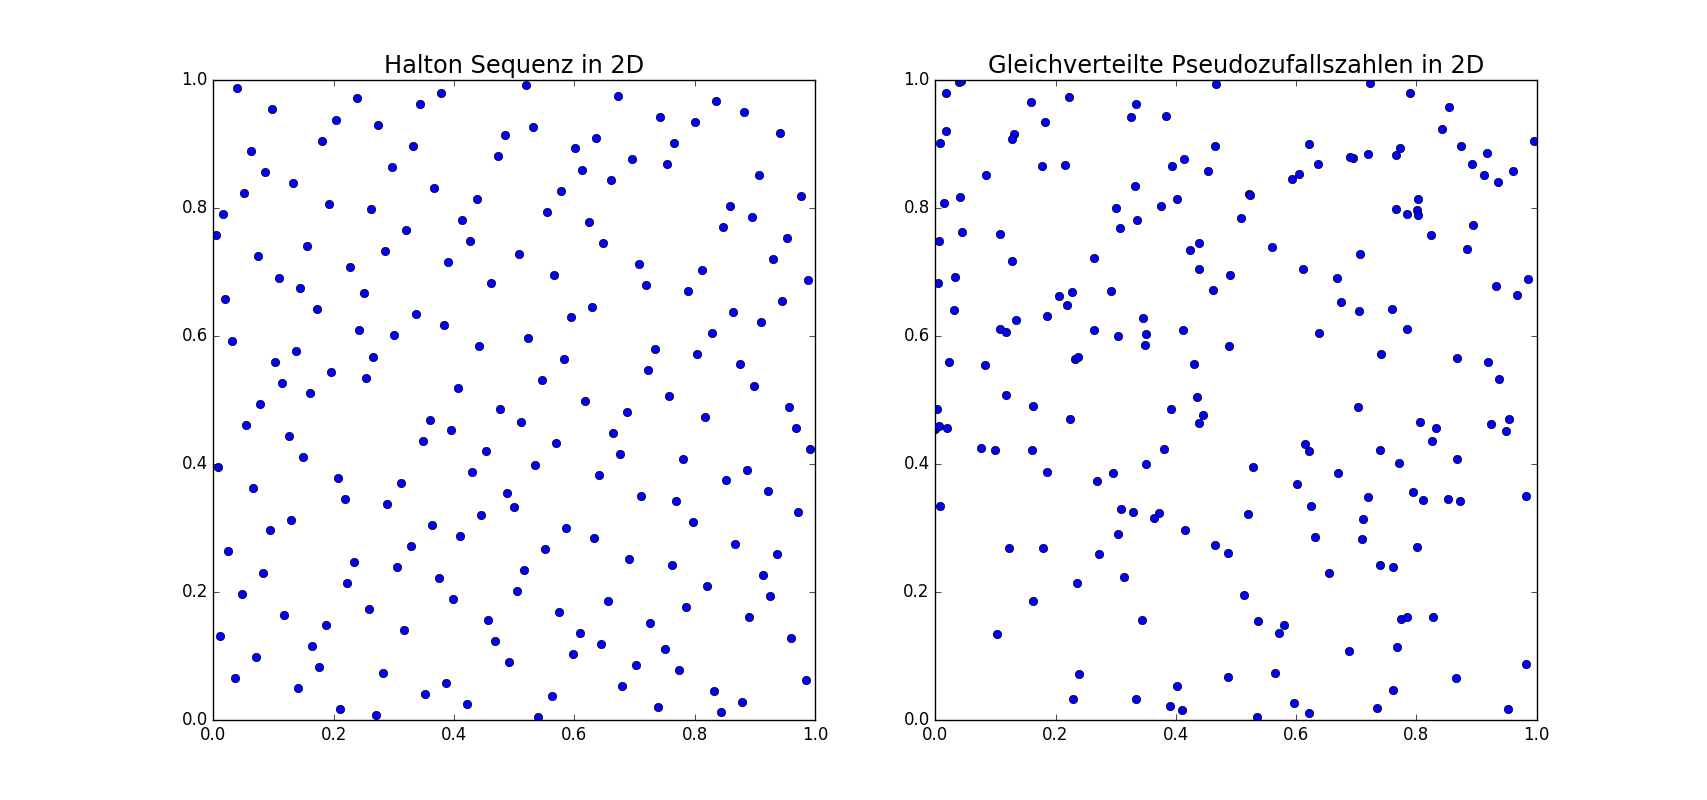
\includegraphics[width=\textwidth]{Figures/halton_numbers.png}
\caption{Darstellung der ersten 200 Halton Zahlen im zweidimensionalen und im Vergleich 200 gleichverteilte Pseudozufallszahlen. Die Halton Sequenz deckt die Fläche dabei viel gleichmäßiger ab.}
\label{fig:halton_numbers}
\end{figure}
Benötigt man wiederum Zufallszahlen mit einer anderen Verteilungsfunktion, so sind diese durch Anwendung der Inversionsmethode \ref{thinversionsmethode} erzeugbar.

\subsection{Approximation von Erwartungswert und Varianz}
Bevor wir den Kern der Schleife betrachten, wollen wir uns zuerst mit den eng miteinander zusammenhängenden Fragen \ref{mcsaveresults} und \ref{mcestimations} beschäftigen. Diese Fragen über die Verwendung der einzelnen Zwischenergebnisse zur Approximation des Erwartungswertes und der Varianz können wiederum vielseitig beantwortet werden.
\subsubsection*{Verarbeitung am Ende}
Gegeben sei ein Zeitpunkt $T>0$ und die stochastische KGG (\ref{skgg}) zu einer Zufallsvariablen $Y$ und gesucht seien $\E[u(T,x,Y)]$ und $\text{var}(u(T,x,Y))$. Sind für $i=1,\dots,R$ die deterministischen Lösungen $u_i(T,x,y_i)$ gespeichert, so verwenden wir als Approximationen
\begin{align*}
\E[u(T,x,Y)]&\approx \frac{1}{R}\sum_{i=1}^R u_i(T,x,y_i)\eqqcolon m_R\\
\text{var}(u(T,x,Y)) &\approx \frac{1}{R-1}\sum_{i=1}^R(u_i(T,x,y_i)-m_R)^2
\end{align*}
Wieso diese Approximationen sinnvoll sind, zeigt sich teilweise aus dem zentralen Grenzwertsatz \ref{thzentralgrenzwert}. Es folgt für unabhängige Stichproben $y_i$ die Aussage \[\sqrt{R}(m_R-\E[u(T,x,Y)])\xrightarrow{R\to\infty}\mathcal{N}(0,\text{var}(u(T,x,Y)))\]
und schlussendlich 
\[m_R=\E[u(T,x,Y)] + \mathcal{O}\left(\frac{1}{\sqrt{R}}\right)\]
In welchem Konvergenz Sinne die letzte Aussage zu verstehen ist und welche Faktoren dabei in den letzten Term einfließen, sei an dieser Stelle nicht weiter ausgeführt. Wir werden diese Konvergenzordnung in Beispielen jedoch empirisch bestätigen.\\[0.2cm]
Die für die Approximation der Varianz verwendete Darstellung nennt man auch \emph{korrigierte Stichprobenvarianz}. Sie ist ein erwartungstreuer Schätzer der Varianz einer Stichprobe und ein Werkzeug aus der Statistik, welches wir hier nicht weiter erläutern werden.
\subsubsection*{Fortlaufende Berechnung}
Die Verarbeitung am Ende besitzt zwei große Nachteile:
\begin{itemize}
\item Sämtliche Zwischenergebnisse müssen gespeichert werden. Für die Mittelwertbildung alleine wäre dies zwar nicht nötig, jedoch für die Approximation der Varianz. An einer Beispielsrechnung soll der benötigte Arbeitsspeicher kurz verdeutlicht werden: Wird der Raum in 256 Punkten diskretisiert und benötigt jeder Punkt 8 Byte Speicher und führt man (durchaus realistisch) $R=100000$ Simulationen durch, so ergibt sich bereits ein Speicherbedarf von $\frac{256*100000*8\text{B}}{1024^2}\approx 200\text{MB}$. Dies ist also bereits für eine räumliche Dimension ein nicht unerheblicher Aufwand.
\item Die Methode zur Approximation der Varianz ist nicht stabil und stark anfällig für numerische Rechenfehler, insbesondere Überläufe (vgl. \autocite{cook08}). Aus diesem Grunde schlug Welford in \autocite{welford62} eine alternative Berechnungsmethode vor, welche wir im folgenden erklären werden.
\end{itemize}
\begin{maththeorem}
\label{thiterativemk}
Für $x_1,\dots,x_k\in\R$ und $m_k=\frac{1}{k}\sum_{j=1}^kx_j$ gilt für $k\in\N$ die iterative Darstellung
\[m_k=m_{k-1}+\frac{x_k-m_{k-1}}{k},\quad \text{mit }\: m_0=0\]
\end{maththeorem}
\begin{proof}
Wir zeigen mithilfe vollständiger Induktion die äquivalente Aussage, dass die Rekursion mit der Darstellung $m_k=\frac{1}{k}\sum_{j=1}^kx_j$ übereinstimmt.\\
I.A. ($k=1$): \[m_1=0+\frac{x_1-0}{1}=x_1=\sum_{j=1}^1x_j\quad\surd\]
I.S. ($k\leadsto k+1$):
\begin{align*}
m_{k+1}&\stackrel{Def}{=}m_k+\frac{x_{k+1}-m_k}{k+1}\\
&\stackrel{IV}{=}\frac{1}{k}\sum_{j=1}^kx_j+\frac{x_{k+1}}{k+1}-\frac{1}{k(k+1)}\sum_{j=1}^kx_j
\end{align*}
Multiplizieren wir nun mit $k(k+1)$ so erhalten wir
\begin{align*}
k(k+1)m_{k+1}&=(k+1)\sum_{j=1}^kx_j+kx_{k+1}-\sum_{j=1}^kx_j\\
&=k\sum_{j=1}^{k+1}x_j\\
\implies m_{k+1}&=\frac{1}{k+1}\sum_{j=1}^{k+1}x_j
\end{align*}
\end{proof}
Wir haben nun also eine iterative Methode zur Berechnung des Mittelwertes gewonnen, die nur den vorherigen Mittelwert, die neue Stichprobe und die Anzahl an Stichproben benötigt. Diese Methode ist robust gegen Überläufe und numerisch stabil. Viel wichtiger ist jedoch die iterative Berechnung des Varianzschätzers, welche auf ähnlichen Ideen basiert. Die Äquivalenz zur ursprünglichen Methode ist dabei allerdings schwieriger zu erkennen.
\begin{maththeorem}
Für $x_1,\dots,x_k\in\R$, $m_k$ wie in Satz \ref{thiterativemk} und $s_k=\sum_{j=1}^k(x_j-m_k)^2$ gilt für $k\in\N$ die iterative Darstellung
\[s_k=s_{k-1}+(x_k-m_k)(x_k-m_{k-1}),\quad\text{mit }s_0=0\]
\end{maththeorem}
\begin{proof}
Es gilt für $j<k$ wegen $m_k=\frac{k-1}{k}m_{k-1}+\frac{1}{k}x_k$
\begin{align}
x_j-m_k&=x_j-m_{k-1}+\frac{1}{k}m_{k-1}-\frac{1}{k}x_k \nonumber\\
\label{eqn:mcvar1}
&=x_j-m_{k-1}-\frac{1}{k}(x_k-m_{k-1})\tag{*}\\
\label{eqn:mcvar2}
x_k-m_k&=\frac{k-1}{k}(x_k-m_{k-1})\tag{**}
\end{align}
Dann gilt für $k\in\N$
\begin{align*}
s_k&=\sum_{j=1}^k(x_j-m_k)^2\stackrel{(\ref{eqn:mcvar2})}{=}\sum_{j=1}^{k-1}(x_j-m_k)^2+\frac{(k-1)^2}{k^2}(x_k-m_{k-1})^2\\
&\stackrel{(\ref{eqn:mcvar1})}{=}\sum_{j=1}^{k-1}(x_j-m_{k-1})^2-\frac{2}{k}(x_k-m_{k-1})\sum_{j=1}^{k-1}(x_j-m_{k-1})+\frac{k-1}{k^2}(x_k-m_{k-1})^2\\
&\quad +\frac{(k-1)^2}{k^2}(x_k-m_{k-1})^2\\
&=s_{k-1}-\frac{2}{k}(x_k-m_{k-1})\underbrace{\left((k-1)m_{k-1}-(k-1)m_{k-1}\right)}_{=0}+\underbrace{\frac{(k-1)^2+k-1}{k^2}}_{=\frac{k-1}{k}}(x_k-m_{k-1})^2\\
&=s_{k-1}+\frac{k-1}{k}(x_k-m_{k-1})\underbrace{(x_k-m_{k-1})}_{\stackrel{(\ref{eqn:mcvar2})}{=}\frac{k}{k-1}(x_k-m_k)}=s_{k-1}+(x_k-m_{k-1})(x_k-m_k)
\end{align*}
\end{proof}
Teilen wir nun $s_k$ noch durch $k-1$, so erhalten wir wieder die korrigierte Stichprobenvarianz. Wir benötigen dafür nur den vorherigen Wert $s_{k-1}$, die beiden letzten Mittelwerte, die neuste Stichprobe $x_k$ und die Stichprobenanzahl.
\subsection{Numerische Ergebnisse}
Man bemerkt schon an der Pseudocode Darstellung der Monte-Carlo-Methode, dass das Bottleneck des Algorithmus in der Berechnung der Lösung der deterministischen KGG liegt. Der Zeitaufwand für alle anderen Operationen ist in Relation dazu vernachlässigbar klein. Ein großer Vorteil des Algorithmus ist seine \emph{embarrassingly parallel} Eigenschaft: Es ist quasi kein Aufwand nötig die Schleife zu parallelisieren und somit skaliert er perfekt mit der Anzahl an zur Verfügung stehenden Prozessoren. Dies ist eine erste Antwort auf Frage \ref{mcalgspeed}, jedoch sollte klar sein, dass das Lösen des deterministischen Systems dennoch so effizient wie möglich passieren muss. Ein Löser, der nur 0.1 Sekunden für ein einziges System benötigt und $R=100000$ Durchgänge erledigt, läuft bereits etwa 3 Stunden ohne Parallelisierung.\\
\subsubsection*{Konvergenz}
Anhand von Abbildung \ref{fig:mc_convergence_trial1} erkennen wir für Beispiel \ref{bsp:trial1} die (probabilistische) Konvergenz des Erwartungswertes und der Varianz mit ungefährer Ordnung $0.5$ für die Monte-Carlo-Methode. Vergleichen wir dazu die Quasi-Monte-Carlo-Methode anhand desselben Beispiels in Abbildung \ref{fig:quasi_mc_convergence_trial1}, so erkennen wir eine bessere Konvergenzordnung und ein weniger chaotisches Verhalten des Fehlers.\\
Diese schlechte Konvergenzordnung macht das Verfahren sehr unattraktiv. Wir benötigen selbst für das simple Beispiel \ref{bsp:trial1} und die Quasi-Monte-Carlo-Methode bereits $R=100000$ Durchläufe für einen Fehler des Erwartungswertes in die Größenordnung $10^{-5}$.
\begin{figure}
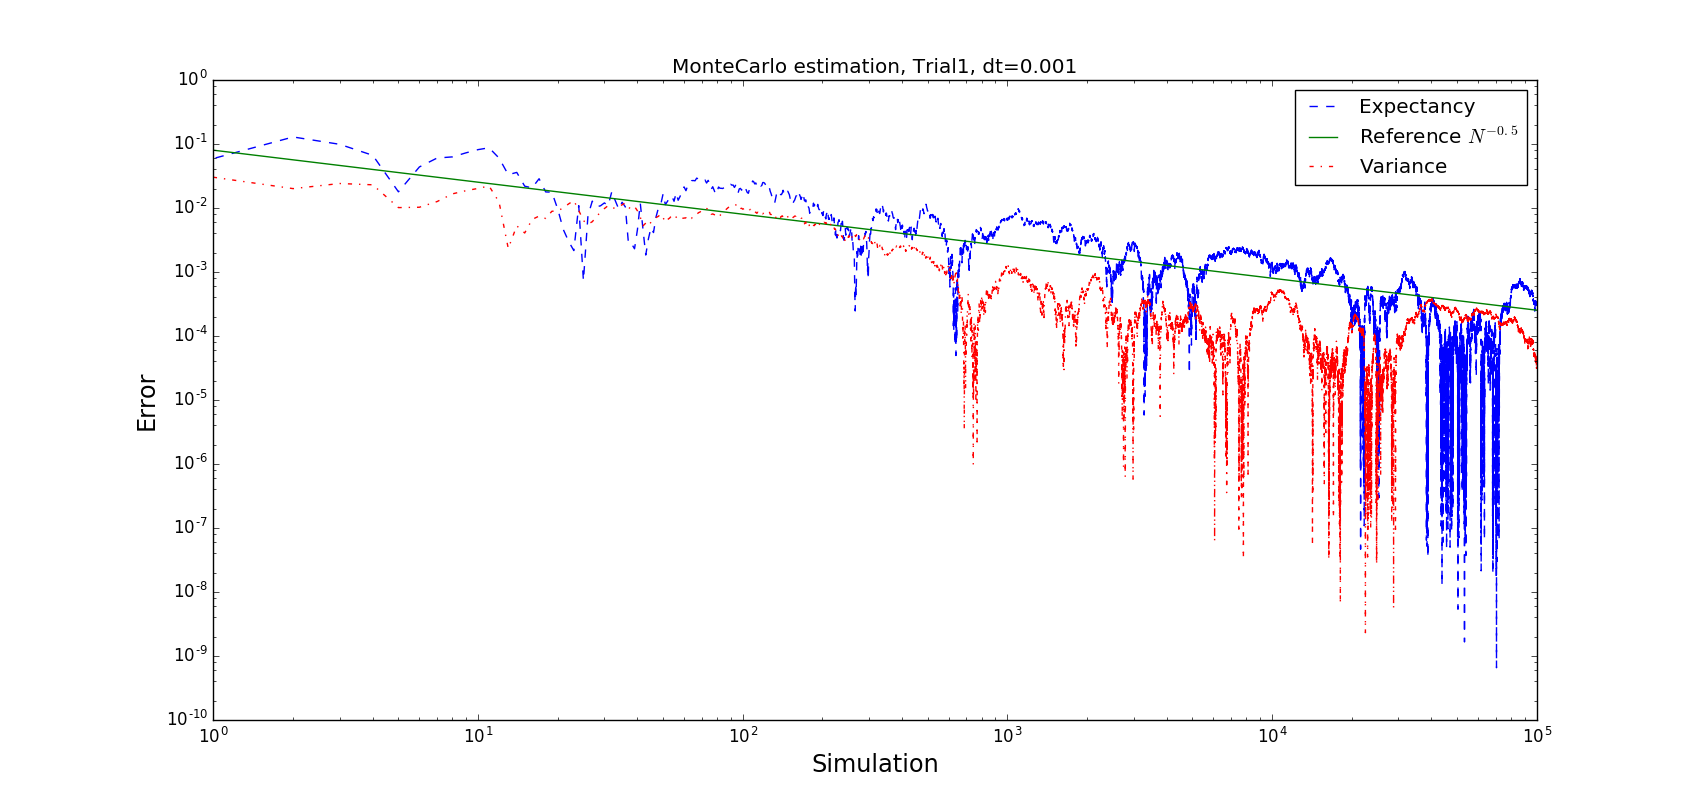
\includegraphics[width=\textwidth]{Figures/mc_convergence_trial1.png}
\caption{Konvergenz des Erwartungswertes und der Varianz von Beispiel \ref{bsp:trial1} mithilfe der Monte-Carlo-Methode zum Zeitpunkt $T=0.5$. Ordnungsplot mit Referenzlinie $0.08\frac{1}{\sqrt{R}}$ der erwarteten Ordnung.}
\label{fig:mc_convergence_trial1}
\end{figure}\\
\begin{figure}
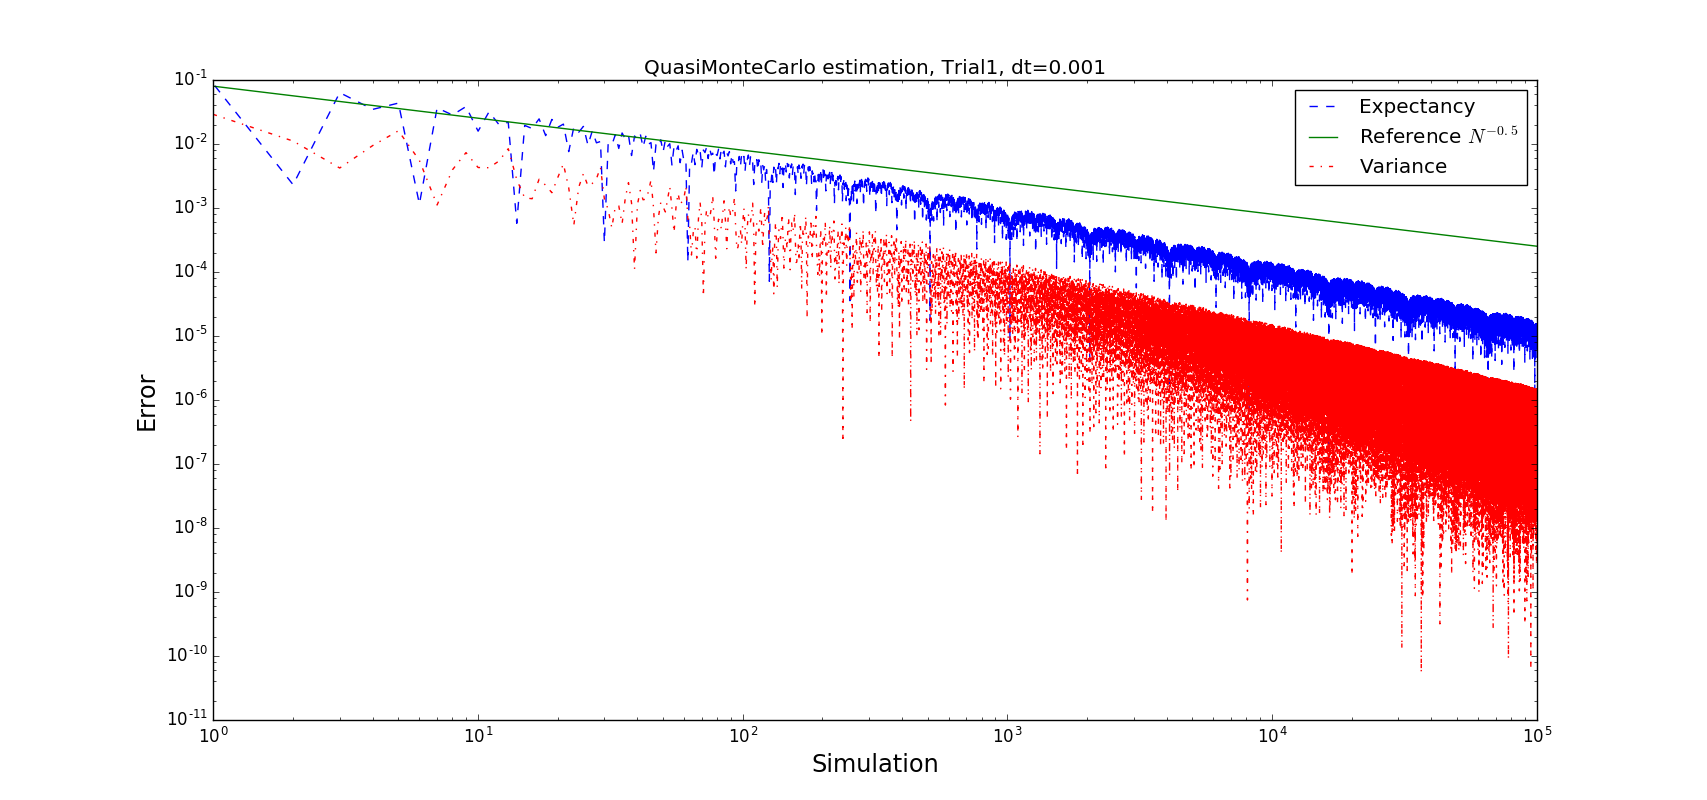
\includegraphics[width=\textwidth]{Figures/quasi_mc_convergence_trial1.png}
\caption{Konvergenz des Erwartungswertes und der Varianz von Beispiel \ref{bsp:trial1} mithilfe der Quasi-Monte-Carlo-Methode zum Zeitpunkt $T=0.5$. Ordnungsplot mit Referenzlinie $0.08\frac{1}{\sqrt{R}}$.}
Einen Vorteil allerdings bietet das Verfahren: Unabhängig von der Größe des Zufallsvektors $Y$ erhalten wir jeweils dieselbe Konvergenzordnung und benötigen bis auf die Generierung der Komponenten keinen zeitlichen Mehraufwand für die Ausführung des Algorithmus im Vergleich zu eindimensionalen Zufallsvektoren. Diese Eigenschaft wird von keinem anderen Verfahren, das wir noch vorstellen werden geteilt. Im Gegenteil nämlich wird der Rechenaufwand exponentiell in der Größe des Zufallsvektors steigen. 
\label{fig:quasi_mc_convergence_trial1}
\end{figure}
\todo[inline]{Bilder: Konvergenzordnung von MC anhand von bsp1 und 2; Zeige bessere Ordnung und Fehlerverhalten von qMC; Zeige Konvergenzordnung von Varianz; Zeige was R=100000 so bedeutet im Vergleich zu R=317=sqrt(100000); Erwähne Vorteil dass Konvergenz unabhäng von Dim. von y (zeige entsprechendes BSP)}

 
% Chapter 3

\chapter{Stochastische Collocation}
\todo[inline]{Interpolation;Quadratur (Xiu Kap7) mit Gauß, Glenshaw-Curtis; smolyak sparse grids (fully nested failed, weakly nested and non nested; discrete projection;Äquivalenz von Interpol + diskr proj (zumindest mal in 1d, mehr bei entspr nodes/weights?)}
% Chapter 4

\chapter{Stochastische Kollokation}
\label{Chapter4}
Wie bereits die Monte-Carlo-Methode basieren auch stochastische Kollokationsverfahren auf \emph{sampling}, d.h. der wiederholten Auswertung von vielen Zufallsexperimenten. Bei der Monte-Carlo-Methode werden die Punkte der gegebenen Verteilung entsprechend unabhängig und zufällig gewählt. Die Konvergenz ist in einem stochastischen Sinne durch das Gesetz der großen Zahlen gegeben.\\
Dies ist ein großer Unterschied zu den hier vorgestellten stochastischen Kollokationsverfahren. Für diese werden die Kollokationspunkte nicht zufällig, sondern so gewählt, dass mithilfe von ihnen eine Polynominterpolation oder Quadratur möglich ist. Konvergenz ist dann abhängig davon, wie gut sich die stochastische Größe durch Polynome von Zufallsvariablen approximieren lässt.\\
Die beiden Ansätze \emph{Interpolation} und \emph{diskrete Projektion} (auch \emph{pseudospektraler Ansatz} genannt) werden für die stochastische KGG im Folgenden detailliert vorgestellt und miteinander verglichen.
\section*{Kollokation für die stochastische KGG}
Die stochastische KGG (\ref{skgg}) für $d$ räumliche Dimensionen, $N$ stochastische Dimensionen und $y\in\R^N$ ist definiert durch
\begin{align*}
\partialdtt{u}(t,x,y)&=\alpha(y) \Laplace_x u(t,x,y) - \beta(x,\omega)u(t,x,y), \: t>0, \, x\in \Torus^d\\
u(0,x,y)&=u_0(x,y), \: x\in \Torus^d\\
\partialdt{u}(0,x,y)&=v_0(x,y), \: x\in \Torus^d
\end{align*}
Im klassischen Sinne bedeutet Kollokation, dass eine Approximation für eine diskrete Knotenmenge $\Theta_Y=\lbrace y_i\in\R^N\mid i=1,\dots,S\rbrace$ exakt ist. Auf die stochastische KGG übertragen muss also für $y=y_i\in\Theta_Y$ die Lösung $u(t,x,y_i)$ für $x\in\Torus^d$ und $t>0$ vorliegen und die Approximation $w$ erfüllt $w(t,x,y_i)=u(t,x,y_i)$ für $i=1,\dots,S$. Da wir die exakte Lösung $u(t,x,y_i)$ nicht kennen, sondern für einen Zeitpunkt $T>0$ und eine Knotenmenge $\lbrace x_j\in\Torus^d\mid j=1,\dots,H\rbrace$ nur eine Approximation $\tilde{u}$ berechnen können (z.B. mithilfe des Strang-Splittings), gilt für festes $x_j$ die Kollokationsbedingung lediglich approximativ:
\[w(T,x_j,y_i)=u(T,x_j,y_i)\approx \tilde{u}(T,x_j,y_i),\quad i=1,\dots,S\]
Wir wählen daher $\tau$ so klein, dass dieser Fehler im Vergleich zum eigentlichen Kollokationsfehler vernachlässigbar gering ist. Zur Vereinfachung der Notation nehmen wir im Folgenden an, die Lösung $u(T,x_j,y_i)$ liege exakt vor.

\section{Interpolation}
Sei $Y$ ein $N$-dimensionaler Zufallsvektor mit stochastisch unabhängigen Komponenten und $\Theta_Y\subset \mathcal{J}_Y$ eine $S$-elementige Knotenmenge. Seien weiter $\lbrace \Phi_m \mid |m|\le P \rbrace$ die gPC Basisfunktionen zu $Y$ und im Folgenden mit $m=0,\dots,M=\binom{N+P}{P}-1$ durchnummeriert. Eine Diskussion zur Nummerierung findet man im vorherigen Kapitel.\\
Dann wählen wir als Interpolationspolynom die Funktion
\begin{equation}
\label{eqn:coll_interpol_basic}
w_M^{(j)}(Y)=\sum_{m=0}^M\hat{w}_m^{(j)}\Phi_m(Y)\in\Poly_P^N(Y),\quad j=1,\dots,H
\end{equation}
und fordern als Interpolationsbedingung
\[w_M^{(j)}(y_i)=u(T,x_j,y_i),\quad i=1,\dots,S, j=1,\dots,H\]
Die Notation macht klar, dass wir zu einem gegebenen Zeitpunkt $T>0$ und jedem festen Knotenpunkt $x_j$ die stochastische Funktion $u(T,x_j,Y)$ durch ein Polynom in $Y$ approximieren wollen.\\
Betrachten wir die Gleichung (\ref{eqn:coll_interpol_basic}) in den Knotenpunkten $y_i$ für jedes $i=1,\dots,S$, so können wir das entstehende System kompakt schreiben als
\begin{equation}
\label{eqn:interpol_compact}
A\hat{w}=u
\end{equation}
mit 
\begin{align*}
A&=(\Phi_m(y_i))_{i=1,\dots,S;m=0,\dots,M}\in\R^{S\times (M+1)}\\
\hat{w}&=(\hat{w}_m^{(j)})_{m=0,\dots,M;j=1,\dots,H}\in\R^{(M+1)\times H}\\
u&=(u(T,x_j,y_i))_{i=1,\dots,S;j=1,\dots,H}\in\R^{S\times H}\\
\end{align*}
Für jeden Knotenpunkt $x_j$ ist ein lineares Ausgleichsproblem der Größe $S\times (M+1)$ zu lösen. Ist $S\neq M+1$, so verwenden wir die Moore-Penrose-Inverse $A^+$ von $A$ definiert durch
\[A^+\coloneqq \lim\limits_{\delta\to 0}(A^TA+\delta I)^{-1}A^T\]
Dann minimiert $\hat{w}\coloneqq A^+u$ den Ausdruck $\norm{Aw-u}_2$.\\
Ist $S=M+1$ und $A$ regulär, so gilt $A^+=A^{-1}$ und $\hat{w}$ ist die eindeutige Lösung des linearen Gleichungssystems.\\[0.2cm] 
Die obige Schreibweise erlaubt es in vielen Programmiersprachen die Systeme gleichzeitig zu lösen und bietet somit einen starken Laufzeitvorteil gegenüber dem Lösen von $H$ separaten Gleichungen. Um sicherzustellen, dass das System nicht unterbestimmt ist, muss gelten $S\ge M+1=\binom{N+P}{P}$. Später werden wir an verschiedenen Beispielen Konsequenzen dieser Bedingung genauer betrachten.
\begin{mathbem}
In Gleichung (\ref{eqn:gpc_approx_exp}) wurde gezeigt, dass sich der Erwartungswert an der Stelle $x_j$ approximieren lässt durch
\[\E[u(t,x_j,Y)]\approx \hat{w}_0^{(j)}\]
Da die Gleichungen gekoppelt sind, müssen aber trotzdem auch alle anderen $\hat{w}_m$ berechnet werden.
\end{mathbem}
\subsection{Wahl der Interpolationspunkte}
\label{chapter:interpolation_points}
Wir wollen direkt am Anfang darauf hinweisen, dass im Mehrdimensionalen für $N>1$ die Wahl der Knotenpunkte für die Interpolation ein nicht vollständig verstandenes Problem darstellt. Im Eindimensionalen existieren die Lagrangepolynome, die es ermöglichen ein Interpolationspolynom zu jeder beliebigen Knotenmenge zu definieren. Das Konzept der Lagrange-Interpolation lässt sich wie in \autocite{San07} gezeigt konzeptuell auf den mehrdimensionalen Fall erweitern. Allerdings benötigt sie die entsprechende Bedingung $\det(A)\neq 0$, welche besagt, dass die Interpolation durch die gegebenen Knotenpunkte eindeutig ist. Die Beziehung dieser Bedingung zur Wahl der Knotenpunkte stellt ein "'komplexes Problem"' dar. Es gibt keine gesicherten Aussagen darüber, dass das volle Tensorprodukt einer eindimensionalen Knotenmenge eine eindeutige Interpolation im Mehrdimensionalen ermöglicht.
\subsubsection*{Grundlagen der eindimensionalen Interpolation}
Der Satz von Cauchy ist ein erster Orientierungspunkt um die Abhängigkeit der Interpolationsgüte von der Wahl der Knotenpunkte für den eindimensionalen Fall und einem kompakten Intervall zu untersuchen.
\begin{maththeorem}[Cauchy]
Sei $f\in C^{S}[-1,1]$ eine $S$ mal stetig differenzierbare Funktion. Dann gibt es für jede Knotenmenge $\lbrace y_1,\dots,y_{S}\rbrace$ ein $\xi\in [-1,1]$, so dass für $y\in[-1,1]$ der Interpolationsfehler gegeben ist durch
\[f(y)-\mathcal{Q}_{S}f=\frac{f^{(S)}(\xi)}{S!}\prod_{i=1}^{S}(y-y_i)\]
Dabei ist $\mathcal{Q}_Sf\in\Poly_S$ das Interpolationspolynom von $f$ mit $\mathcal{Q}_Sf(y_i)=f(y_i)$ für $i=1,\dots,S$.
\end{maththeorem}

Da die Funktion gegeben ist, hat man keinen Einfluss auf die Ableitung $f^{(S)}$. Wegen
\[\norm{f(y)-\mathcal{Q}_{S}f}\le \frac{\norm{f^{(S)}}_\infty}{S!}\underbrace{\norm{\prod_{i=1}^{S}(y-y_i)}}_{=\norm{w(y)}}\]
ist somit das Ziel, den Term $\norm{w(y)}$ abhängig von der Norm zu minimieren.
\begin{mathbem}[\chebyspace Interpolation]
\label{bem:cheby}
Die Nullstellen $y_i=\cos\left(\pi\frac{2i-1}{2S+2}\right)$, für $i=1,\dots,S+1$, der \chebyspace Polynome $T_{S+1}(y)=\cos((S+1)\arccos(y))$ minimieren den Ausdruck $\norm{w(y)}_\infty$ auf $[-1,1]$ und bieten auf $[-1,1]$ optimale Interpolationsgüte. Es gilt 
\[\norm{f(y)-\mathcal{Q}_{S+1}f}_\infty\le \frac{\norm{f^{(S+1)}}_\infty}{2^S(S+1)!}\]
\end{mathbem}
Die \chebyspace Polynome bilden eine Orthogonalbasis bezüglich $\langle \cdot,\cdot\rangle_{L_w^2[-1,1]}$ mit $w(y)=(1-y^2)^{-\onehalf}$. Eine Idee ist es nun, auch Nullstellen anderer orthogonalen Polynombasen als Knotenpunkte zu verwenden um ähnliche Approximationsergebnisse auf nicht-kompakten Intervallen zu erhalten.
\begin{maththeorem}
\label{th:interpol_and_proj}
Sei $\lbrace \Phi_m\in\Poly_m\mid m=0,\dots,M\rbrace\subset L_w^2(\mathcal{J})$ eine Orthonormalbasis von Polynomen und $(y_i,a_i)_{i=0,\dots,M}$ eine Quadraturformel mit Exaktheitsgrad $2M$ bezüglich $w$ und $y_i\neq y_j,i\neq j$, d.h. alle Polynome $p\in\Poly_{2M}$ vom Grad kleiner gleich $2M$ werden mit dem Gewicht $w$ exakt integriert:
\[\int_\mathcal{J} p(y)w(y)dy=\sum_{i=0}^M a_ip(y_i)\]
Sei weiter das Interpolationspolynom  $\mathcal{Q}_Mf$ einer Funktion $f\colon \mathcal{J}\to\R$ bezüglich den Interpolationspunkten $\lbrace y_i\mid i=0,\dots,M\rbrace$ beschrieben durch
\[\mathcal{Q}_Mf(y)=\sum_{m=0}^M\hat{w}_m\Phi_m(y)\]
Die Koeffizienten $\hat{w}_m$ werden in Analogie zu (\ref{eqn:interpol_compact}) berechnet durch das Lösen des linearen Gleichungssystems
\[A\hat{w}=\hat{f}\]
Dann ist \[\hat{w}_i=\sum_{j=0}^M\Phi_i(y_j)a_jf(y_j)\approx \int_\mathcal{J} \Phi_i(y)f(y)w(y)dy,\quad i=0,\dots,M\]
\end{maththeorem}
\begin{proof}
Es ist $A_{ij}=\Phi_j(y_i)$. Da wir uns im eindimensionalen Fall befinden ($N$=1) ist die Vandermonde-artige Matrix $A$ invertierbar, da die $\Phi_i$ eine Basis bilden und die $y_i$ paarweise verschieden sind. Es gilt für $\widetilde{w}_i\coloneqq \sum_{j=0}^M\Phi_i(y_j)a_jf(y_j)$ und $\widetilde{w}\coloneqq (\widetilde{w}_i)^T$
\begin{align*}
\left(A\widetilde{w}\right)_i&=\sum_{j=0}^M\Phi_j(y_i)\widetilde{w}_j\\
&=\sum_{j=0}^M\Phi_j(y_i)\sum_{k=0}^M\Phi_j(y_k)a_kf(y_k),\quad \text{Interpol.:} f(y_k)=\sum_{\ell=0}^M\hat{w}_\ell\Phi_\ell(y_k)\\
&=\sum_{\ell=0}^M\hat{w}_\ell \sum_{j=0}^M\Phi_j(y_i)\sum_{k=0}^M\Phi_j(y_k)a_k\Phi_\ell(y_k)\\
&\stackrel{\text{deg}(\Phi_j\Phi_\ell)\le 2M}{=}\sum_{\ell=0}^M\hat{w}_\ell\sum_{j=0}^M\Phi_j(y_i)\underbrace{\int_\mathcal{J}\Phi_j(y)\Phi_\ell(y)w(y)dy}_{=\delta_{j\ell}}\\
&=\sum_{\ell=0}^M\hat{w}_\ell\Phi_\ell(y_i)=f(y_i)=\hat{f}_i
\end{align*}
Also gilt $A\widetilde{w}=\hat{f}=A\hat{w}$. Da $A$ eine reguläre Matrix ist folgt schlussendlich $\widetilde{w}=\hat{w}$.
\end{proof}
\begin{mathbem}
Wir wollen nun dem technischen Satz \ref{th:interpol_and_proj} Leben einhauchen und seine Relevanz verdeutlichen.
\begin{itemize}
\item
Die vorausgesetzte Existenz einer Quadraturformel mit $M+1$ verschiedenen Quadraturpunkten und Exaktheitsgrad $2M$ ist durch die später vorgestellte Gauss-Quadratur erfüllt. Die Quadraturpunkte sind dabei die Nullstellen des $M+1$-ten Basispolynoms und daher paarweise verschieden. Die Quadraturgewichte lassen sich über die erste Komponente des zugehörigen normierten Eigenvektors der Matrix aus dem Golub-Welsch-Algorithmus (siehe kommende Bemerkung \ref{bem:gaussquad}) bestimmen.
\item
Wir sehen, dass sich im Eindimensionalen bei bekannter Quadraturformel die Interpolationskoeffizienten $\hat{w}_m$ auch einzeln ohne Lösen eines linearen Gleichungssystems berechnen lassen. Diese Darstellung führt auf den später vorgestellten zweiten Ansatz zur stochastischen Kollokation.
\item
Die Darstellung $\hat{w}_i=\sum_{j=0}^M\Phi_i(y_j)a_jf(y_j)$ kann als Approximation an die Koeffizienten $\int_\mathcal{J} \Phi_i(y)f(y)w(y)dy$ der Bestapproximation $P_Mf$ in $L_w^2(\mathcal{J})$ aufgefasst werden. Mithilfe der Dreiecksungleichung lässt sich dann der Fehler der Interpolation beschreiben durch
\begin{align*}
&\norm{\mathcal{Q}_Mf-f}_{L_w^2}\le \underbrace{\norm{P_Mf-f}_{L_w^2}}_{\text{Fehler der Bestapproximation}}+\underbrace{\norm{\mathcal{Q}_Mf-P_Mf}_{L_w^2}}_{\text{Aliasing-Fehler}}\\
&=\norm{\mathcal{Q}_Mf-P_Mf}_{L_w^2}+\norm{\sum_{m=0}^M\left(\sum_{j=0}^M\Phi_m(y_j)a_jf(y_j)\right)\Phi_m-\sum_{m=0}^M\left(\int_\mathcal{J}\Phi_m(y)f(y)w(y)dy\right)\Phi_m}_{L_w^2}\\
&=\norm{\mathcal{Q}_Mf-P_Mf}_{L_w^2}+\norm{\sum_{m=0}^M\left(\sum_{j=0}^M\Phi_m(y_j)a_jf(y_j)-\int_\mathcal{J}\Phi_m(y)f(y)w(y)dy\right)\Phi_m}_{L_w^2}\\
&\stackrel{\text{Parseval}}{=}\norm{\mathcal{Q}_Mf-P_Mf}_{L_w^2}+\sqrt{\sum_{m=0}^M\left(\sum_{j=0}^M\Phi_m(y_j)a_jf(y_j)-\int_\mathcal{J}\Phi_m(y)f(y)w(y)dy\right)^2}
\end{align*}
Schlussendlich lässt sich also der Fehler der Interpolation durch den Fehler der Bestapproximation in $L_w^2$ und einen Quadraturfehler bezüglich der Gewichtsfunktion $w$ beschreiben. Für den Fehler der Bestapproximation erwarten wir nach Xiu spektrale Konvergenz. Finden wir eine zur Gewichtsfunktion $w$ passende Quadraturformel, so hat lediglich die Glattheit von $f$ Einfluss auf den Quadraturfehler, da $\Phi_m$ als Polynom bei hinreichend hoher Ordnung exakt integriert wird.
\end{itemize}
\end{mathbem}
\begin{mathbsp}
Wir vergleichen anhand von \nameref{trial:1} für $d=1$ zwei Möglichkeiten zur Wahl der Interpolationspunkte. Da $Y$ eine Gleichverteilung zugrunde liegt, verwenden wir die normalisierten Legendre-Polynome $L_0,\dots,L_M$ als gPC Basis Polynome. Als Interpolationspunkte $y_i$ wählen wir dann
\begin{enumerate}
\item die $M+1$ Nullstellen des Legendre-Polynoms vom Grad $M+1$ (genannt \textit{full\_tensor}).
\item die $M+1$ Nullstellen des \chebyspace Polynoms vom Grad $M+1$ (siehe Bemerkung \ref{bem:cheby}).
\end{enumerate}
In Abbildung \ref{fig:Kollokation_trial1} ist die Approximationsgüte der Interpolation dargestellt. Links wird die Zeitschrittweite $\tau=0.001$ für das zugrunde liegende Splittingverfahren verwendet, rechts die Zeitschrittweite $\tau=0.0001$. Die Güte wird gemessen durch die Fehler an den Erwartungswert und die Varianz. Man erkennt, dass die \chebyspace Interpolation langsamer konvergiert als die Legendre-Interpolation. Die Konvergenz stoppt bei einer gewissen Genauigkeit, die abhängig ist von $\tau$. Dies ist dadurch begründet, dass die Punkte $u(T,x_j,y_i)$ nicht exakt vorliegen sondern lediglich mithilfe eines Strang-Splittings mit Schrittweite $\tau$ approximiert werden. Dies betont die Wichtigkeit der Wahl eines kleinen $\tau$, allerdings bedeutet ein kleineres $\tau$ gleichzeitig eine entsprechende multiplikative Vergrößerung der Berechnungszeit.
\begin{figure}[!htb]
\minipage{0.5\textwidth}
  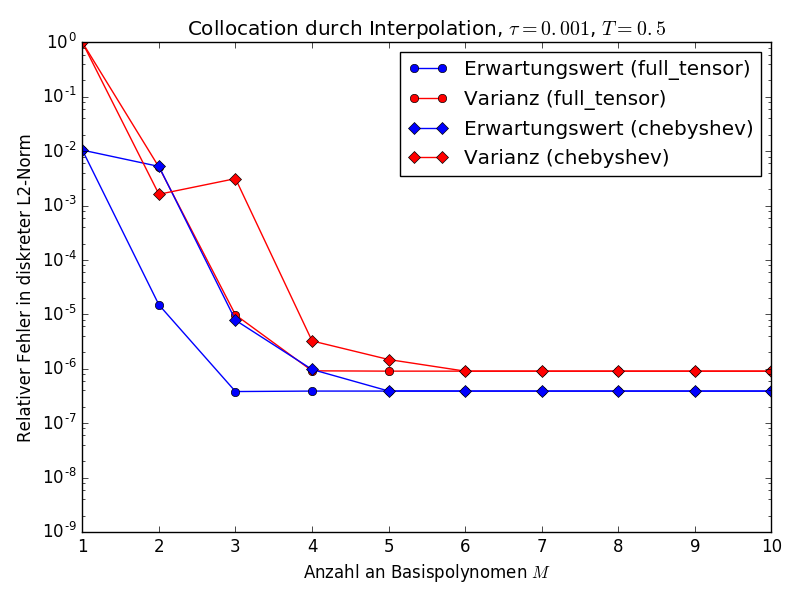
\includegraphics[width=\linewidth]{Figures/collocation_mi_trial1_tau001.png}
\endminipage
\minipage{0.5\textwidth}
  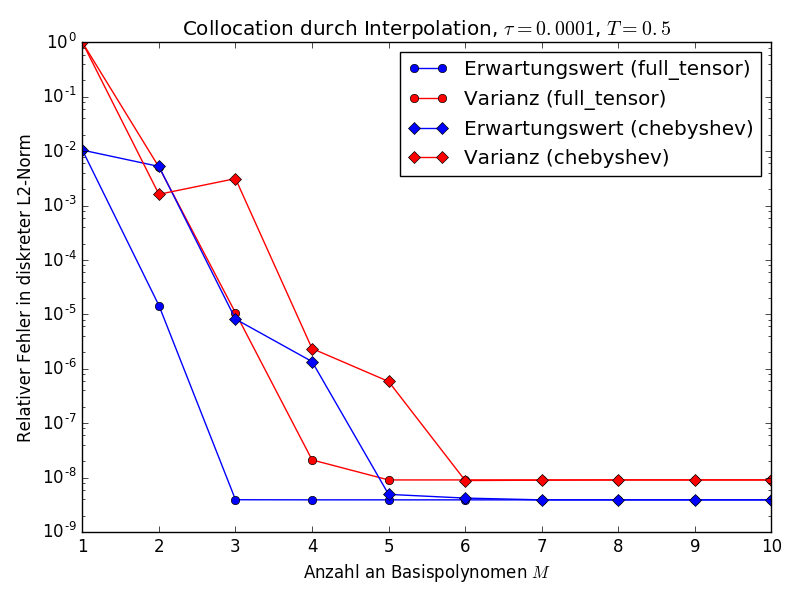
\includegraphics[width=\linewidth]{Figures/collocation_mi_trial1_tau0001.png}
\endminipage
\caption{Vergleich von verschiedenen Interpolationspunkten und der Abhängigkeit der bestmöglichen Interpolation von der Genauigkeit der Interpolationspunkte anhand von \nameref{trial:1} zum Zeitpunkt $T=0.5$ und für $d=1$.}
\label{fig:Kollokation_trial1}
\end{figure}
\end{mathbsp}
\subsubsection*{Mehrdimensionale Interpolation durch volles Tensorprodukt}
Eine Möglichkeit, für $N>1$ die Menge der Interpolationspunkte $\Theta_Y^N$ zu einem gegebenem Zufallsvektor $Y$ der Dimension $N$ zu wählen, ist gegeben durch das volle Tensorprodukt
\[\Theta_Y^N=\Theta_{Y_1}\otimes \dots \otimes \Theta_{Y_N},\quad \Theta_{Y_i}\subset \mathcal{J}_{Y_i}\]
Dann gilt für die Anzahl der Interpolationspunkte $S=S_1 \dots S_N$. Ist die Anzahl an Basispolynomen $M+1$ fest, dann ist es schwierig, die Bedingung $S=M+1$ exakt zu erfüllen. Wir fordern daher, dass $S_1=\dots=S_N$ und $S\ge M+1$ minimal gewählt wird. Dieser Ansatz wird in Abbildungen durch \textit{full\_tensor} gekennzeichnet.
\subsubsection*{Mehrdimensionale Interpolation durch pseudo-dünne Gitter}
Eine weitere Idee für die mehrdimensionale Interpolation, welche die Gleichung $M+1=\binom{N+P}{P}$ exakt erfüllt, ist mit $S_1=\dots=S_N$ die Wahl
\[\Theta_Y^N=\lbrace (y_{m_1},\dots,y_{m_N})\in \Theta_{Y_1}\otimes \dots \otimes \Theta_{Y_N} \mid |m|\le P,m\in\N_0^N \rbrace \]
Es wird somit jedem Multi-Index $m\in\N_0^N$ genau ein mehrdimensionaler Interpolationspunkt $y$ zugewiesen und es gilt $M+1=S$. Die Matrix im Interpolationsansatz ist dadurch quadratisch und besitzt für kleine $P$ eine geringere Kondition als die Matrix aus dem vollen Tensorproduktansatz.\\[0.1cm]
Die Wahl der Nummerierung der eindimensionalen Interpolationspunkte ist entscheidend. Für Legendre- oder Hermite-Polynome bietet sich eine betragsmäßig aufsteigende Sortierung der Punkte an, da diese symmetrisch um $0$ verteilt sind. Für Jacobi- und Laguerre-Polynome beobachten wir in Abbildung \ref{fig:poly_roots} keine Symmetrie. Dennoch gilt die Eigenschaft von Orthogonalpolynomen, dass die Nullstellen eines Polynoms höheren Grades zwischen den Nullstellen des vorherigen Polynoms zu finden sind. Wir sortieren die Nullstellen auf- oder absteigend um eine möglichst repräsentative Auswahl der Punkte des vollen Tensorprodukts zu bekommen. Die Idee ist dadurch motiviert, dass so die Struktur der Entwicklung der Nullstellen einer Polynombasis berücksichtigt wird, auch wenn diese keine eindeutige Schachtelung aufweisen.\\
Dieser Ansatz wird in Abbildungen durch \textit{pseudo\_sparse} gekennzeichnet. Er ist eine Heuristik um den Einfluss der Überbestimmtheit des zu lösenden Systems besser zu verstehen und sollte nicht als robuste Methode für mehrdimensionale Interpolation aufgefasst werden.\\
\begin{figure}[!htb]
\minipage{0.5\textwidth}
  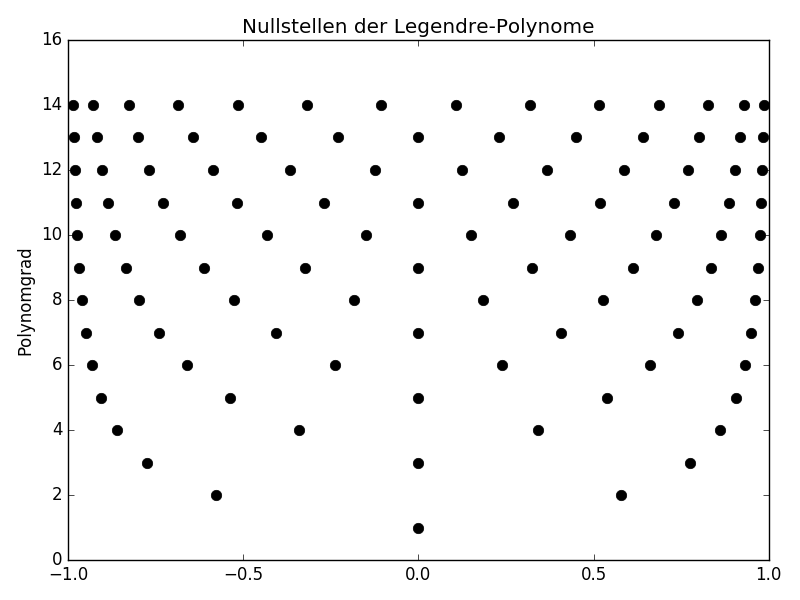
\includegraphics[width=\linewidth]{Figures/roots_legendre.png}
  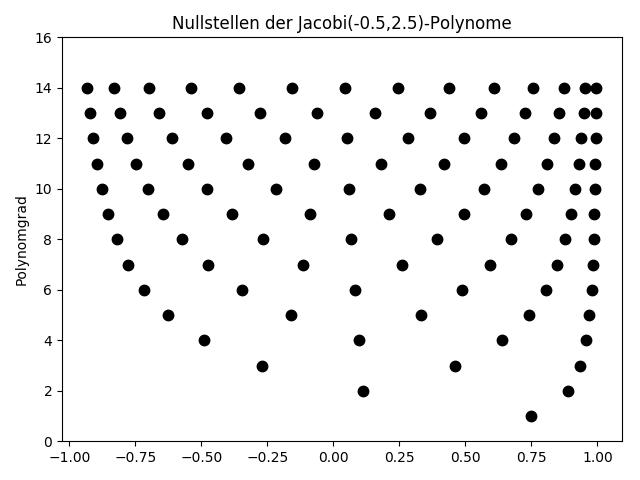
\includegraphics[width=\linewidth]{Figures/roots_jacobi.png}
\endminipage
\minipage{0.5\textwidth}
  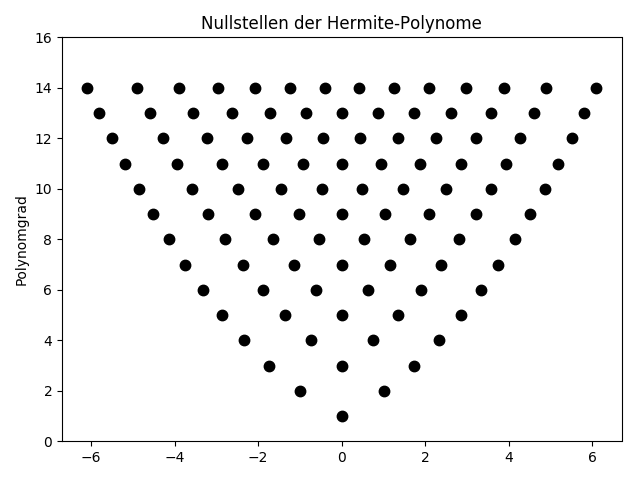
\includegraphics[width=\linewidth]{Figures/roots_hermite.png}
  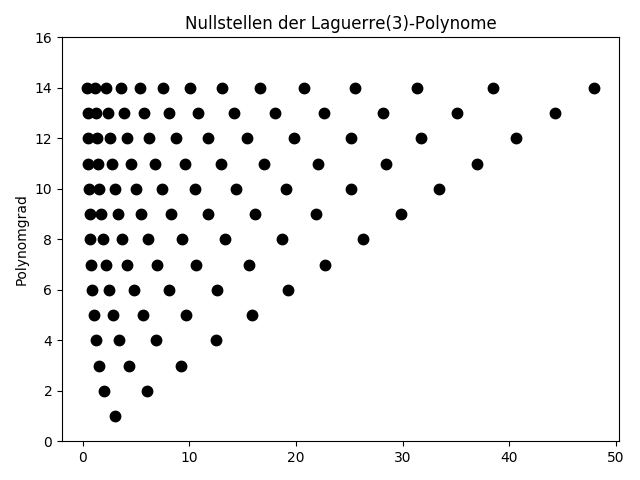
\includegraphics[width=\linewidth]{Figures/roots_laguerre.png}  
\endminipage
\caption{Nullstellen verschiedener Orthogonalbasen von Polynomen mit steigendem Grad.}
\label{fig:poly_roots}
\end{figure}
Ein Beispiel sei für $N=2$ und $P=14$ gemacht, wo für Legendre- und Laguerre-Polynome die Interpolationspunkte des pseudo-dünnen Gitters und des vollen Tensorprodukts in Abbildung \ref{fig:roots_two_dim} dargestellt sind.\\
\begin{figure}[!htb]
\centering
\minipage{0.5\textwidth}
  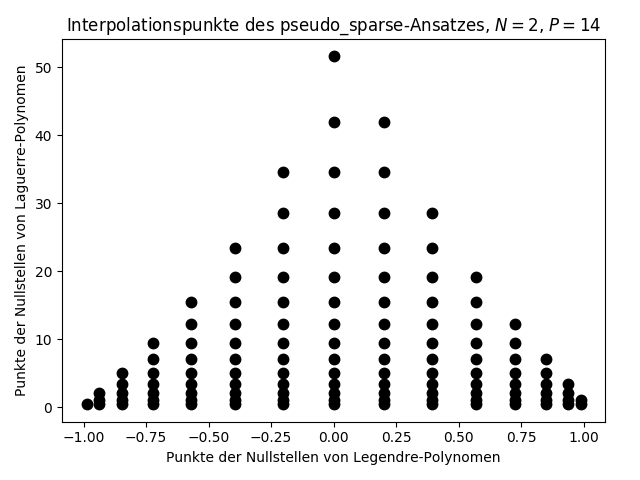
\includegraphics[width=\linewidth]{Figures/roots_pseudo_sparse.png}
\endminipage
\minipage{0.5\textwidth}
  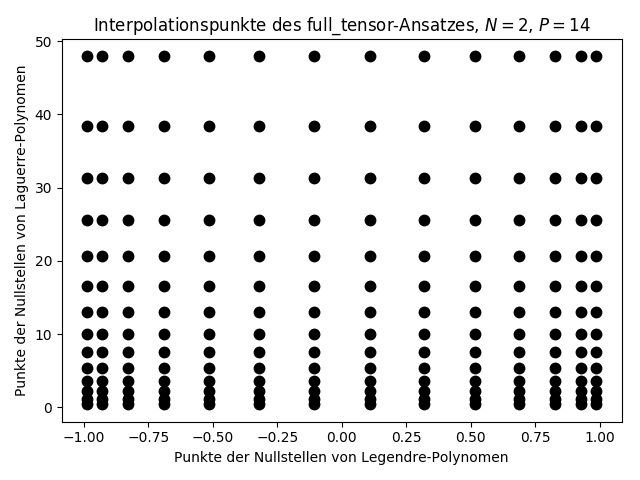
\includegraphics[width=\linewidth]{Figures/roots_full_tensor.png}
\endminipage
\caption{Interpolationspunkte für den pseudo-dünne Gitter Ansatz und das volle Tensorprodukt für die Nullstellen der Legendre- und Laguerre(3)-Polynome mit $N=2$ und $P=14$.}
\label{fig:roots_two_dim}
\end{figure}

Wir werden später basierend auf Smolyaks Konstruktion einen effizienteren Dünngitteransatz kennenlernen, der nicht nur für Interpolation verwendbar ist, sondern sich auch auf generelle Operatoren übertragen lässt. Dieser basiert allerdings auf vollen Tensorprodukten von Operatoren und ist daher nur übertragbar, wenn wir volle Tensorprodukte von Polynombasen zulassen (d.h. ohne die zusätzliche Bedingung $|m|\le P$). Da dies einen erheblichen Rechenaufwand impliziert, werden wir keine Dünngitteransätze für die Interpolation verwenden.
\subsection{Algorithmus}
In Algorithmus \ref{alg:Kollokation_mi} ist das Kollokationsverfahren für den eindimensionalen Fall $d=1$ skizziert. Diese Variante der Kollokation durch Interpolation wird in der Literatur auch mit \emph{Matrix-Invertierung} (MI) bezeichnet. Die Matrix $A$ muss nicht explizit invertiert werden, trotzdem besteht der Kern des Verfahrens aus dem Lösen der linearen Gleichungssysteme bzw. linearen Ausgleichsprobleme.\\
\begin{tabular}{c|c}
Parameter & \\
\hline
$H$ & Anzahl an Punkten der Ortsdiskretisierung\\
$\kappa\in [0,1]$ & Gewicht für das Splittingverfahren zur Approximation von $u(T,x,Y)$\\
$Y$ & $N$-dimensionaler Zufallsvektor zu dem eine gPC-Basis existiert\\
$M+1$ & Anzahl an multivariaten gPC-Basispolynomen\\
$S$ & Anzahl an Interpolationspunkten gemäß einer der möglichen Ansätze
\end{tabular}
\begin{algorithm}[ht]
    \caption{Kollokation durch Interpolation mithilfe von Matrix-Invertierung.}
    \label{alg:Kollokation_mi}
    \begin{algorithmic}[1] % The number tells where the line numbering should start
        \Function{Kollokation\_Interpolation\_MI}{$H, u_0, v_0, \alpha,\beta,\kappa,Y, M, S,\tau, T$} 
            \State $\Phi_m\gets$ $m$-te orthonormale gPC-Basis-Funktion zu $Y$, $\quad m=0,\dots,M$
            \State $y_i\gets$ (multivariate) Interpolationspunkte (siehe Kapitel \ref{chapter:interpolation_points}), $\quad i=1,\dots,S$
            \State $A\gets (\Phi_m(y_i))_{i=1,\dots,S;m=0,\dots,M}\in\R^{S\times M+1}$
            \For{$i=1,\dots,S$}
           		\State $\tilde{u}_{ij}\gets \text{Fast\_Strang}(H,u_0(\cdot, y_i),v_0(\cdot, y_i),\alpha(y_i),\beta(\cdot, y_i),\kappa,\tau,T)_j$
           	\EndFor
            \State $u\gets (\tilde{u}_{ij})_{i=1,\dots,S;j=1,\dots,H}\in\R^{S\times H}$
            \State $\hat{w}\gets A^{-1}u\in\R^{M+1\times H}$
            \State \Comment{Lösen des linearen Ausgleichsproblems, gleichzeitig für alle $u_j$}
			\State $\mu\gets \hat{w}_{0,j=1,\dots,H}$ \Comment{Approximation an Erwartungswert}
			\State $\sigma^2_j\gets \sum_{m=1,\dots,M}\hat{w}^2_{mj}$\Comment{Approximation an Varianz an der Stelle $x_j$}
			\State \textbf{return} $\mu,\sigma^2$ \Comment{Approximation an Erwartungswert und Varianz}        
        \EndFunction
    \end{algorithmic}
\end{algorithm}
\subsection{Vergleiche der Ansätze}
Wir beschränken uns für $N=1$ auf die Nullstellen derjenigen Orthogonalpolynome, die gemäß des gPC zu der Verteilung von $Y$ gehören. Für das kompakte Intervall $\mathcal{J}=[-1,1]$ wäre es ebenso möglich, die \chebyspace Interpolationspunkte zu verwenden. Diese bieten aber nach unseren Beobachtungen keinen Vorteil.\\
Für $N>1$ besteht die Möglichkeit, das volle Tensorprodukt der jeweiligen eindimensionalen Interpolationspunkte zu den Komponenten von $Y$ zu wählen. Da dies jedoch im Allgemeinen mehr Punkte umfasst als die vorhandenen $M+1$ Polynome, ist das lineare Gleichungssystem überbestimmt und wir beobachten eine hohe Kondition der Matrix. Die Invertierbarkeit der Matrix für die mehrdimensionale Interpolation ist selbst im quadratischen Fall nicht garantiert. Dies sorgt insbesondere dafür, dass die Approximation der Varianz, welche jede Komponente des Lösungsvektors benötigt, bereits für $P>3$ instabil ist.\\
Anhand der \nameref{trial:8} aus dem Appendix mit $N=4$ vergleichen wir die beiden Ansätze in Abbildung \ref{fig:Kollokation_trial8}. 
\begin{figure}[!htb]
\centering
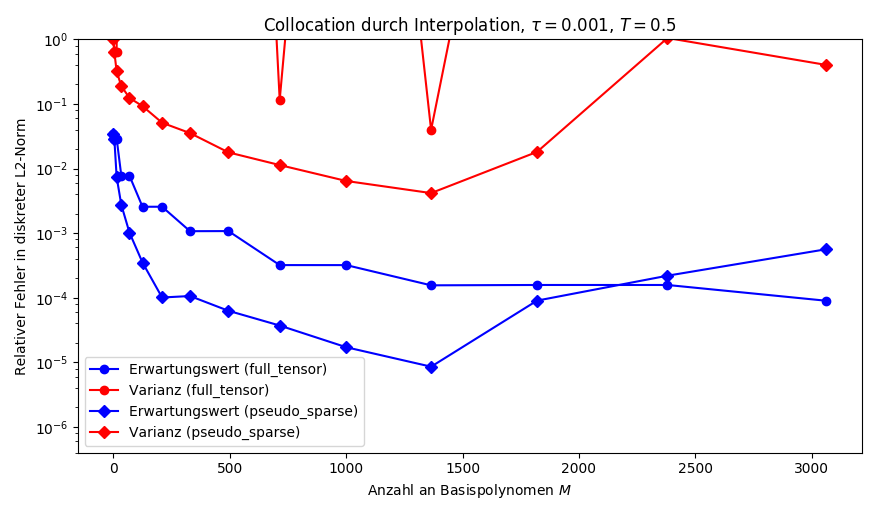
\includegraphics[width=\linewidth]{Figures/collocation_mi_trial8_ft_pseudosparse.png}
\caption{Approximation des Erwartungswerts und der Varianz von \nameref{trial:8} mithilfe von Kollokation durch Interpolation (also gemäß Gleichung (\ref{eqn:interpol_compact})) und verschiedene Ansätze zur Wahl der Interpolationspunkte bis zu $P=14$.}
\label{fig:Kollokation_trial8}
\end{figure}
Wir sehen, dass sich der Erwartungswert mit beiden Ansätzen approximieren lässt. Bis zu $P=11$ ist die Approximation mit dem pseudo\_sparse Ansatz dabei um einen Faktor 10 genauer. Die Kondition der Matrix ist für $P=11$ jedoch bereits in der Größenordnung $\mathcal{O}(10^{13})$ mit wachsender Tendenz, was Approximationen mit $P>11$ zunehmend schlechter werden lässt.\\
Die Varianz ist durch das überbestimmte System beim full\_tensor Ansatz nicht berechenbar (für $P=9$ ergibt sich ein System der Größe $6^4\times \binom{4+9}{9} =1296\times 715$). Erhöht man $P$ weiter, so beobachtet man auch für den pseudo\_sparse Ansatz zunehmende Instabilität.

\section{Diskrete Projektion}
\label{sec:discrete_proj}
Der zweite Ansatz zur stochastischen Kollokation basiert auf der Bestapproximation in $L_{\rho_Y}^2$.
\begin{mathdef}[Diskrete Projektion]
Sei $Y$ ein Zufallsvektor und $\Phi_m(Y)$ für $m=0,\dots,M$ die zugehörigen orthonormalen gPC Basisfunktionen. Dann ist die Bestapproximation der sKGG zu einem Zeitpunkt $T>0$ und für eine Stelle $x_j$ definiert als
\[P_Mu(T,x_j,Y)=\sum_{m=0}^M\hat{u}_m^{(j)}\Phi_m(Y)\]
mit Koeffizienten
\[\hat{u}_m^{(j)}=\E[u(T,x_j,Y)\Phi_m(Y)]=\int_{\mathcal{J}_Y} u(T,x_j,y)\Phi_m(y)\rho_Y(y)dy\]
Ist nun $(y_i,a_i)_{i=0,\dots,Q}$ eine Quadraturformel für das Gewicht $\rho_Y$, so ist die diskrete Projektion definiert als
\[w_{M,Q}(T,x_j,Y)=\sum_{m=0}^M\hat{w}_m^{(j)}\Phi_m(Y)\] wobei für die Koeffizienten gilt
\[\hat{w}_m^{(j)}=\sum_{i=0}^Qu(T,x_j,y_i)\Phi_m(y_i)a_i\approx \int_{\mathcal{J}_Y} u(T,x_j,y)\Phi_m(y)\rho_Y(y)dy\]
\end{mathdef}
Satz \ref{th:interpol_and_proj} zeigt, dass für $Q=M$ und eine Quadraturformel mit paarweise verschiedenen Quadraturpunkten und Exaktheitsgrad $2M$ die beiden Ansätze im Eindimensionalen äquivalent sind. Aus der Bemerkung nach Satz \ref{th:interpol_and_proj} folgt auch, dass sich der Fehler der diskreten Projektion mithilfe der Dreiecksungleichung durch den Fehler der Bestapproximation und einen Quadraturfehler, den Aliasing-Fehler, abschätzen lässt.

\subsection{Gauss-Quadratur im Eindimensionalen}
Wir wollen nun eine möglichst exakte Quadraturformel konstruieren, welche auf natürliche Weise das jeweilige Gewicht $\rho$ des Integrals berücksichtigt.
\begin{maththeorem}[Gauss-Quadratur]
Sei $Q_0,\dots,Q_{n+1}\in L_\rho^2(\mathcal{J})$ eine Orthogonalbasis von Polynomen bezüglich des Gewichts $\rho$. Es sei $\text{deg}(Q_j)=j$ für $j=0,\dots,n+1$. Seien $y_0,\dots,y_n$ die Nullstellen des Polynoms $Q_{n+1}$. Dann ist die Quadraturformel $(y_i,a_i)$ mit 
\[\int_\mathcal{J}f(y)\rho(y)dy\approx \sum_{i=0}^na_if(y_i)\]
und 
\[a_i=\int_\mathcal{J} \rho(y)\underbrace{\prod_{j\neq i} \frac{y-y_j}{y_i-y_j}}_{=\ell_i(y)}dy\]
exakt für alle Polynome vom Grad höchstens $2n+1$.
\end{maththeorem} 
\begin{proof}[Beweisskizze]
Sei $f$ ein Polynom vom Grad höchstens $2n+1$ und 
\[f(y)=Q_{n+1}(y)\underbrace{p(y)}_{deg \le n}+\underbrace{r(y)}_{deg \le n}\]
eine durch Polynomdivision erhaltene Zerlegung von $f$. Da die $y_i$ Nullstellen von $Q_{n+1}$ sind, gilt
\[f(y_i)=r(y_i),\quad i=0,\dots n\]
Dann ist
\[\int_\mathcal{J}f(y)\rho(y)dy=\underbrace{\int_\mathcal{J}Q_{n+1}(y)p(y)\rho(y)dy}_{=0}+\int_\mathcal{J}r(y)\rho(y)dy\]
da $Q_{n+1}$ orthogonal zum Raum aller Polynome vom Grad höchstens $n$ ist.\\
Die interpolatorischen Quadraturformeln (wie beispielsweise die Newton-Cotes-Formeln) mit den Gewichten $a_i$, die über das gewichtete Integral der Lagrange-Polynome $\ell_i$ definiert werden, sind exakt für Polynome vom Grad höchstens $n$. Somit gilt
\[\int_\mathcal{J}f(y)\rho(y)dy=\int_\mathcal{J}r(y)\rho(y)dy=\sum_{i=0}^{n}a_ir(y_i)=\sum_{i=0}^{n}a_if(y_i)\]
\end{proof}
\begin{mathbem}
\label{bem:gaussquad}
Wir nennen an dieser Stelle noch einige praktische Hinweise zur Gauss-Quadratur.
\begin{itemize}
\item Die Gauss-Quadraturformel zur entsprechenden gPC Basis erfüllt die Voraussetzungen an die Quadraturformel von Satz \ref{th:interpol_and_proj}.
\item Die Nullstellen $y_i$ lassen sich als die Eigenwerte einer symmetrischen Tridiagonalmatrix mithilfe des Golub-Welsch-Algorithmus (siehe Satz \ref{golubwelschalg}) berechnen.
\item Die Gewichte $a_i$ lassen sich ebenfalls mithilfe des Golub-Welsch-Algorithmus berechnen. Ist $y_i$ ein Eigenwert der symmetrischen Tridiagonalmatrix $J$ mit normalisiertem Eigenvektor $z$, d.h. $Jz=y_iz$ und $\norm{z}=1$, so gilt
\[a_i=(z_1)^2\]
Das Gewicht ist somit das Quadrat des ersten Eintrags des Eigenvektors, siehe \autocite{GolubWelsch}.
\end{itemize}
\end{mathbem}
\subsection{Mehrdimensionale Quadratur}
\label{chapter:multivariatequad}
Um den Ansatz der diskreten Projektion für einen mehrdimensionalen Zufallsvektor mit $N>1$ durchzuführen, benötigen wir eine mehrdimensionale Quadratur. Im Gegensatz zur mehrdimensionalen Interpolation liegt die Schwierigkeit nicht nur darin, eine Menge von Kollokationspunkten zu finden, sondern auch die zugehörige Menge der Quadraturgewichte zu bestimmen.\\
Die numerischen Möglichkeiten der mehrdimensionalen Integration (engl. \emph{cubature}) umfassen unter anderem adaptive Verfahren und Monte-Carlo-Methoden. Da diese auf einer großen Menge an Funktionsauswertungen basieren und in unserem Fall eine Funktionsauswertung das aufwändige Lösen einer Instanz der sKGG bedeutet, benötigen wir somit angepasste Integrationsverfahren.
\subsubsection*{Tensorkonstruktion}
Sei $Y$ ein Zufallsvektor und $L_{Y_i}$ ein eindimensionaler Quadraturoperator bezüglich des Gewichts $\rho_{Y_i}$, beispielsweise die Gauss-Quadratur. Dann erhalten wir mithilfe einer Tensorkonstruktion die mehrdimensionale Quadratur
\[L_Y=L_{Y_1}\otimes\dots\otimes L_{Y_N}\]
Für die Menge an Quadraturpunkten gilt wie schon bei der Interpolation
\[\Theta_Y=\Theta_{Y_1}\otimes\dots\otimes \Theta_{Y_N}\]
Die Anzahl der Quadraturpunkte $Q=Q_1\dots Q_N$ wächst daher wiederum sehr stark. Dies macht den Ansatz bereits für geringe Dimensionen $N$ sehr rechenaufwändig. Andererseits sehen wir sofort, dass sich die polynomiale Exaktheit der Gauss-Quadraturen direkt auf den mehrdimensionalen Fall übertragen lässt. Die Quadratur $L_Y$ ist exakt für alle Polynome in
\[\Poly_{2Q_1-1}(Y_1)\otimes\dots\otimes\Poly_{2Q_N-1}(Y_N)\]
\subsubsection*{Smolyaks dünne Gitter}
Basierend auf \autocite{ConradMarzouk} geben wir eine kurze Einführung in die Konstruktion von Smolyaks dünnen Gittern. Sei $L_{Y_i}^{Q_i}$ ein linearer Operator für die $i$-te Komponente von $Y$. Im Folgenden wird $L_{Y_i}^{Q_i}$ einen Quadraturoperator darstellen, die Konstruktion ist aber beispielsweise auch für Interpolationsoperatoren gültig.\\
Es sei $L_{Y_i}^{Q_i}\to L_{Y_i}$ für $Q_i\to\infty$ konvergent zum entsprechenden exakten Operator. Im Fall der Quadratur bedeutet dies für glatte integrierbare Funktionen $f\colon \mathcal{J}\to\R$
\[L^Qf=\sum_{j=0}^Q a_jf(y_j)\xrightarrow[]{Q\to\infty}\int_\mathcal{J}f(y)dy=Lf\]
Dann lässt sich der exakte Operator als Teleskopsumme darstellen
\[L_{Y_i}=\sum_{m=0}^\infty L_{Y_i}^m - L_{Y_i}^{m-1}=\sum_{m=0}^\infty \varDelta_{Y_i}^m\]
mit $\varDelta_{Y_i}^0=L_{Y_i}^0=0$ und $\varDelta_{Y_i}^m=L_{Y_i}^m-L_{Y_i}^{m-1}$.\\
Wir können das volle Tensorprodukt der exakten Operatoren mithilfe der Teleskopsummen schreiben und Produkt und Summe tauschen
\begin{align*}
L_{Y_1}\otimes\dots\otimes L_{Y_N}&=\sum_{m_1=0}^\infty \varDelta_{Y_1}^{m_1}\otimes\dots\otimes \sum_{m_N=0}^\infty\varDelta_{Y_N}^{m_N}\\
&=\sum_{m\in\N_0^N} \varDelta_{Y_1}^{m_1}\otimes\dots\otimes \varDelta_{Y_N}^{m_N}\\
\end{align*}
Zur Approximation ersetzt man die Summe über alle Multi-Indices $m\in\N_0^N$ durch eine passende Teilmenge. Dazu verwenden wir die Menge aller Indices mit $|m|\le \ell$ und dem Level $\ell$. Schreibt man die Approximation wieder bezüglich der Komponenten $L_{Y_i}^{m_i}$ so gilt nach \autocite{NoTeWe07}
\begin{align*}
L_Y^\ell &= \sum_{|m|\le \ell} \varDelta_{Y_1}^{m_1}\otimes\dots\otimes \varDelta_{Y_N}^{m_N}\\
&= \sum_{\ell - N+1\le |m|\le \ell} (-1)^{\ell - |m|}\binom{N-1}{\ell - |m|}L_{Y_1}^{m_1}\otimes\dots\otimes L_{Y_N}^{m_N}\\
\end{align*}
Die Menge an benötigten Kollokationspunkten ist dann 
\[\Theta_Y^\ell=\bigcup_{\ell - N+1\le |m|\le \ell} \Theta_{Y_1}^{m_1}\times\dots\times \Theta_{Y_N}^{m_N}\]
Die Gestalt und Größe der Menge $\Theta_Y^\ell$ ist abhängig davon, wie die Teilmengen geschachtelt (engl. \emph{nested}) sind. Dies ist eine entscheidende Bedingung für eine eventuelle Reduktion der benötigten Kollokationspunkte. In Abbildung \ref{fig:grids} sehen wir zwei Beispiele für dünne Gitter. Die zugrunde liegenden Knotenmengen $\Theta_{Y_1}^j$ und $\Theta_{Y_2}^j$ sind dabei die Nullstellen der Legendre- bzw. Hermite-Polynome mit Grad $j$.
\begin{figure}[!htb]
\minipage{0.5\textwidth}
  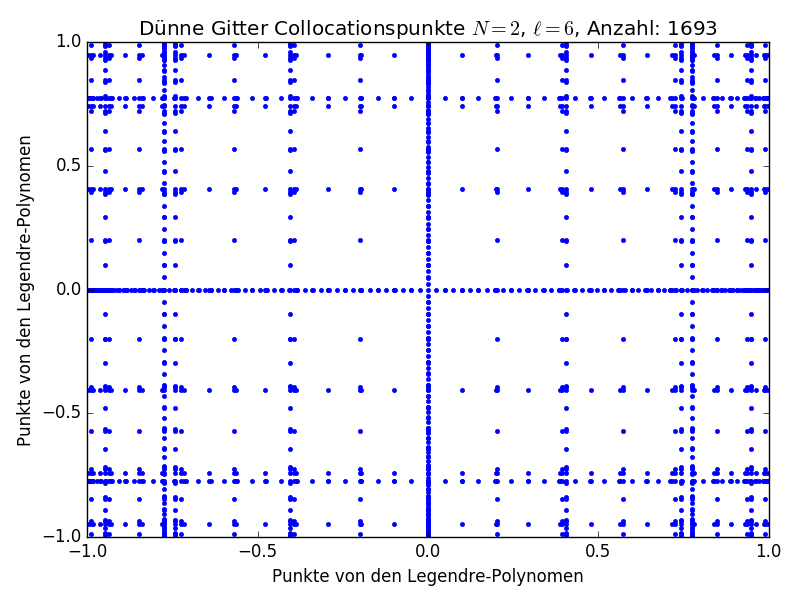
\includegraphics[width=\linewidth]{Figures/sparse_grid_legendre_legendre.png}
\endminipage
\minipage{0.5\textwidth}
  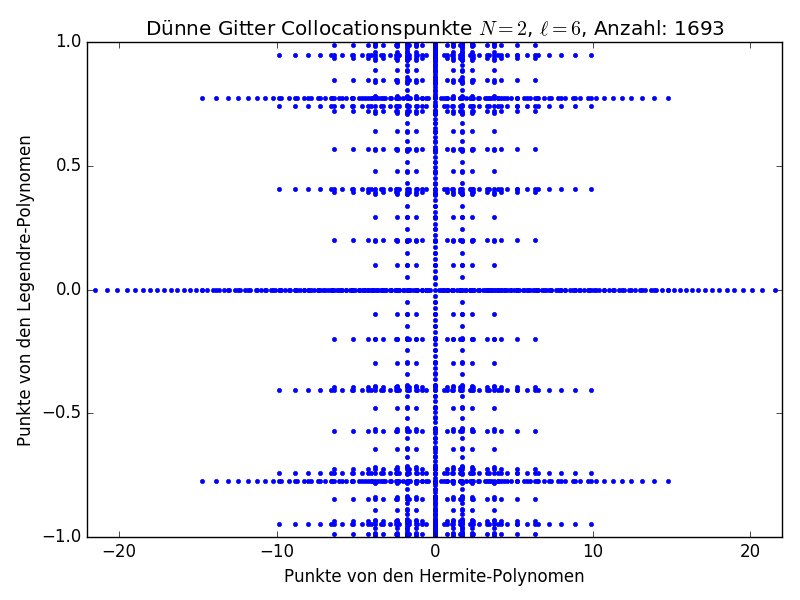
\includegraphics[width=\linewidth]{Figures/sparse_grid_hermite_legendre.png}
\endminipage
\caption{Dünne Gitter nach Smolyak mit $N=2$ und Legendre- bzw. Hermite-Kollokationspunkten für das Level $\ell=6$.}
\label{fig:grids}
\end{figure}
Die Nullstellen der Legendre- und Hermite sind schwach geschachtelt (engl. \emph{weakly nested}), da für ungerade Polynomgrade die Zahl $0$ eine Nullstelle ist. Dies ist jedoch die einzige Wiederholung eines Knotenpunktes. Die Nullstellen der Laguerre- und Jacobi-Polynome besitzen im Allgemeinen keinerlei Schachtelung.\\
Im Gegensatz zu Gittern, die beispielsweise auf Glenshaw-Curtis Knotenpunkten basieren und vollständig geschachtelt sind, bieten schwach geschachtelte Gitter somit wenig Zeitersparnis durch Wiederverwendung von Kollokationspunkten. Der Vorteil liegt hauptsächlich in der geschickten Approximation des vollen Tensorprodukts der exakten Operatoren.\\
Eine Implementierung für vollständig geschachtelte, schwach geschachtelte und nicht geschachtelte dünne Gitter in Matlab und C++ ist durch die Sandia-Sparse-Bibliothek (siehe \autocite{Sandia}) gegeben. Die Schwierigkeit liegt dabei darin, für schwach geschachtelte Gitter die einzelnen wieder auftauchenden Knotenstellen korrekt zu identifizieren.
\begin{figure}[!htb]
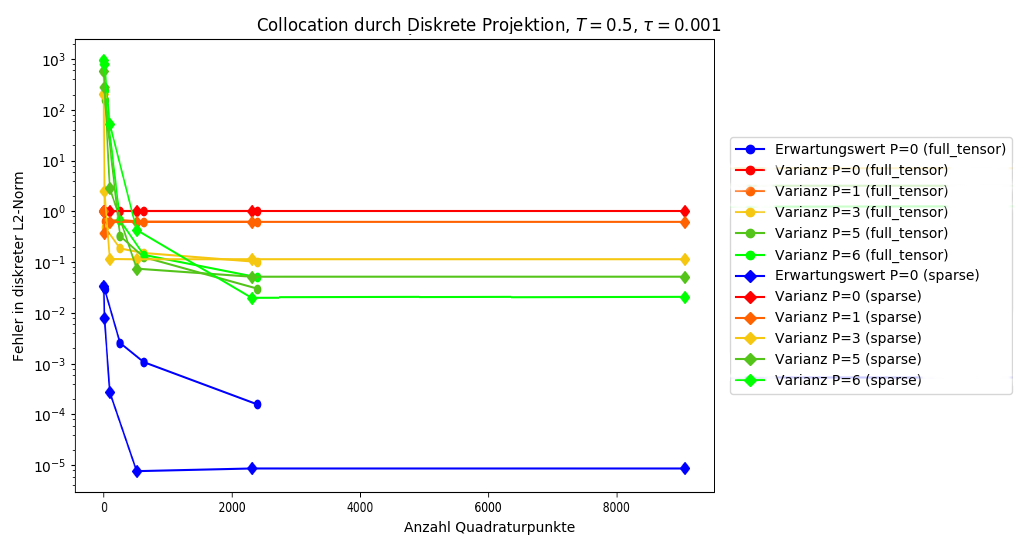
\includegraphics[width=\textwidth]{Figures/collocation_dp_trial8_nebeneinander.png}
\caption{Konvergenz des Erwartungswert und der Varianz mit diskreter Projektion für \nameref{trial:8} mit $N=4$.}
\label{fig:dp_trial8}
\end{figure}
In Abbildung \ref{fig:dp_trial8} wird für \nameref{trial:8} die Konvergenz der diskreten Projektion für das volle Tensorprodukt und den Dünngitteransatz miteinander verglichen. Der Fehler wird dabei in Abhängigkeit von den Anzahl an benötigten Quadraturpunkten gezeigt. Wir beobachten:
\begin{itemize}
\item Der Erwartungswert benötigt nur $P=0$ und ist lediglich abhängig von der Güte der verwendeten Quadraturformel.
\item Der Dünngitteransatz nach Smolyak ist für den Erwartungswert mit 1000 Quadraturpunkten in der Referenzgenauigkeit $\mathcal{O}(10^{-5})$ auskonvergiert.
\item Die maximal mögliche Genauigkeit der Varianz ist abhängig von $P$. 
\item Für größeres $P$ ist der Fehler der Varianz geringer, allerdings gilt dies erst, wenn die Quadraturformel die zusätzlich unter dem Integral auftauchenden Polynome $\Phi_m$ für $|m|=P$ exakt integriert.
\item Bei der Varianz zeigt der Dünngitteransatz keine klaren Vorteile, da der Gesamtfehler stärker von $P$ als vom Quadraturfehler abhängig ist.
\item Will man die Varianz besser approximieren, so benötigt man mehr Koeffizienten $\hat{w}_m^{(j)}=\sum_{i=0}^Qu(t,x_j,y_i)\Phi_m(y_i)a_i$. Dies bedeutet, dass die Quadratur häufiger berechnet werden muss. Die Kollokationsstellen $u(t,x_j,y_i)$, die unabhängig von $m$ sind, können allerdings wieder verwendet werden.
\end{itemize} 

\subsubsection*{Glenshaw-Curtis-Quadratur}
Die Glenshaw-Curtis-Quadratur basierend auf den Knotenpunkten 
\[y_i=\cos\left(\frac{(n-1-i)\pi}{n-1}\right)\in[-1,1],\quad n\ge 2, i=0,\dots,n-1\]
ist eine häufig genutzte Quadraturformel mit vollständig geschachtelten Quadraturpunkten. Die Gewichte lassen sich in $\mathcal{O}(n\log n)$ Schritten berechnen.\\
Diese Quadratur ist für das kompakte Intervall $[-1,1]$ ausgelegt. Für die Legendre-Polynome und die Jacobi-Polynome mit $\alpha,\beta>0$ stimmt der Träger mit dem Träger der zugehörigen stochastischen Verteilung überein. Es gilt
\[\\E[Y]=\int_{[-1,1]}f(y)\rho(y)dy\approx\sum_{i=0}^Qf(y_i)\rho(y_i)a_i\]
Die Dichte $\rho$ wird hier explizit ausgewertet und ist nicht Teil der Quadraturformel, wie dies bei der Gauss-Quadratur der Fall war.\\
Für Hermite-Polynome mit zugehörigem Träger $(-\infty,\infty)$ bzw. Laguerre-Polynome mit zugehörigem Träger $(0,\infty)$ ist daher eine Transformation des Integrals nötig. Da $[-1,1]$ kompakt ist, existiert aber keine Bijektion zwischen den Mengen. Heuristische Ansätze wie das Ignorieren der Randpunkte und anschließender Verwendung des Transformationssatzes auf $(-1,1)$ liefert schlechte Approximationen.\\
Unseren Beobachtungen nach bietet die Glenshaw-Curtis Quadratur keine Vorteile gegenüber der Gauss-Quadratur. Die polynomiale Exaktheit ist lediglich $n$ bei $n$ Quadraturpunkten und verwendet die Dichtefunktion der Verteilung nicht implizit. Die Dichte muss somit ebenfalls durch die Quadratur approximiert werden, was den nötigen Polynomgrad noch weiter erhöht. Schlussendlich erhöhen die Polynome $\Phi_m$, die bei der Approximation der Varianz unter dem Integral auftauchen, die benötigte polynomiale Exaktheit.
\subsection{Algorithmus}
Algorithmus \ref{alg:Kollokation_dp} skizziert die Berechnung der Approximation von Erwartungswert und Varianz mithilfe von Kollokation durch diskrete Projektion.
\begin{algorithm}[ht]
    \caption{Kollokation durch diskrete Projektion.}
    \label{alg:Kollokation_dp}
    \begin{algorithmic}[1] % The number tells where the line numbering should start
        \Function{Kollokation\_Diskrete\_Projektion}{$H, u_0, v_0, \alpha,\beta,\kappa,Y, M, Q,\tau, T$} 
            \State $\Phi_m\gets$ $m$-te orthonormale gPC-Basis-Funktion zu $Y$, $\quad m=0,\dots,M$
            \State $a_i, y_i\gets$ (multivariate) Quadraturformel (siehe Kapitel \ref{chapter:multivariatequad}), $\quad i=0,\dots,Q$
            \For{$i=1,\dots,S$}
           		\State $\tilde{u}_{ij}\gets \text{Fast\_Strang}(H,u_0(\cdot, y_i),v_0(\cdot, y_i),\alpha(y_i),\beta(\cdot, y_i),\kappa,\tau,T)_j$
           	\EndFor
            \State $\hat{w}_m^{(j)}\gets \sum_{i=0,\dots,Q}\tilde{u}_{ij}\Phi_m(y_i)a_i$
			\State $\mu\gets \hat{w}_{0,j=1,\dots,H}$ \Comment{Approximation an Erwartungswert}
			\State $\sigma^2_j\gets \sum_{m=1,\dots,M}\hat{w}^2_{mj}$\Comment{Approximation an Varianz an der Stelle $x_j$}
			\State \textbf{return} $\mu,\sigma^2$ \Comment{Approximation an Erwartungswert und Varianz}        
        \EndFunction
    \end{algorithmic}
\end{algorithm}
\section{Vergleich der Ansätze Interpolation und diskrete Projektion}
In diesem Abschnitt werden wir die beiden Ansätze für die Kollokation miteinander vergleichen. Dabei werden wir für die Interpolation die Gauss-Stützstellen verwenden und ebenso für die diskrete Projektion die Gauss-Quadratur. Wir betrachten Beispiele mit $N=1$ und $N=4$ und verwenden im mehrdimensionalen Fall den vollen Tensorproduktansatz. Für die mehrdimensionale Quadratur bei der diskreten Projektion vergleichen wir zusätzlich den vollen Tensorproduktansatz mit der Dünngitterquadratur nach Smolyak.
\subsection*{Allgemeiner Vergleich}
\begin{center}
\begin{tabular}{p{0.47\linewidth}|p{0.47\linewidth}}
Interpolation & Diskrete Projektion\\
\hhline{=|=}
\multicolumn{2}{c}{Für Gauss-Stützstellen im Eindimensionalen äquivalent (siehe Satz \ref{th:interpol_and_proj})}\\
\hline
Kollokationspunkte "'beliebig"' & Kollokationspunkte entsprechen Quadraturpunkten\\
\hline
Benötigt Interpolationspunkte & Benötigt zusätzlich Quadraturgewichte zu Quadraturpunkten\\
\hline
Informationen über Stabilität durch Matrixkondition & Explizite Berechnung ohne gekoppeltes System\\
\hline
Erwartungswert abhängig von $P$ & Erwartungswert benötigt nur $P=0$\\
\hline
Bei quadratischer Matrix Varianz nur von $P$ abhängig & Varianz abhängig von $P$ und $Q$\\
\hline
Volles Tensorprodukt macht LGS überbestimmt & Volles Tensorprodukt ohne Stabilitätseinfluss\\
\end{tabular}
\end{center}
Die Überbestimmtheit des Systems bei der Interpolation mit vollem Tensorprodukt der Knoten ist bedingt durch unsere Wahl der Interpolationspolynome. Bei Verwendung des vollen Tensorprodukts der eindimensionalen Polynombasen ist diese Quelle der Instabilität auf Kosten der Rechenzeit beseitigt.\\
Dass für die Berechnung des Erwartungswerts nur $P=0$ benötigt wird, macht die diskrete Projektion für manche Anwendungen sehr attraktiv. Die explizite Berechnung der Koeffizienten, die ohne Lösen eines LGS auskommt, verspricht mehr Stabilität und Geschwindigkeit.\\
Die Beziehung der beiden freien Parameter $P$ für den eindimensionalen Polynomgrad und $Q$ für die Quadraturpunkte ist einerseits aus praktischer Sicht problematisch, da im Vorhinein unklar ist, welche Erhöhung eine Verbesserung der Approximation bietet. Andererseits ist der Einfluss der Parameter auf den Fehler durch die Aufteilung in den Fehler der Bestapproximation und den Aliasing-Fehler aus theoretischer Sicht gut verstanden.
\subsection*{Numerischer Vergleich}

\subsubsection*{Eindimensionaler Fall anhand von \nameref{trial:7}}
Wir sehen in Abbildung \ref{fig:Kollokation_comparison_trial7} für den eindimensionalen Fall die Äquivalenz der diskreten Projektion und der Interpolation bei Verwendung von Nullstellen der orthogonalen Polynome als Kollokationspunkte. Die Äquivalenz ist dann gegeben, wenn die Anzahl verwendeter Polynome $P+1$ der Anzahl verwendeter Quadraturpunkte $Q+1$ entspricht.
\begin{figure}[!htb]
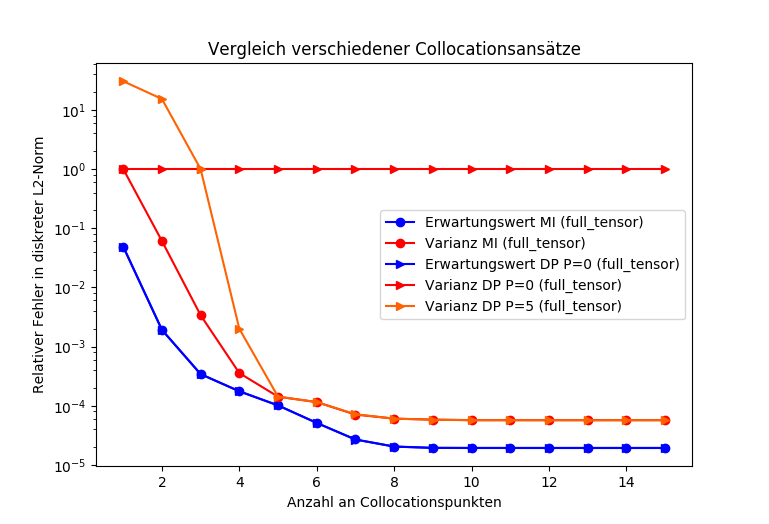
\includegraphics[width=\textwidth]{Figures/collocation_midp_trial7.png}
\caption{Konvergenz der Kollokation für \nameref{trial:7} mit $N=1$ anhand der Anzahl benötigter Kollokationspunkte.}
\label{fig:Kollokation_comparison_trial7}
\end{figure}

\subsubsection*{Vierdimensionaler Fall anhand von \nameref{trial:8}}
Wir sehen in Abbildung \ref{fig:Kollokation_comparison_trial8} den vierdimensionalen Fall. Hier ist der Erwartungswert wiederum für beide Ansätze gleich gut approximierbar unter Verwendung des vollen Tensorprodukts. Die Dünngitterquadratur bietet für den Erwartungswert klare Vorteile in Bezug auf die benötigten Kollokationspunkte.\\
Bei der Interpolation lässt sich die Varianz wegen des überbestimmten Systems nicht zuverlässig berechnen. Bei der diskreten Projektion ist die Konvergenz in $P$ vergleichsweise langsam.
\begin{figure}[!htb]
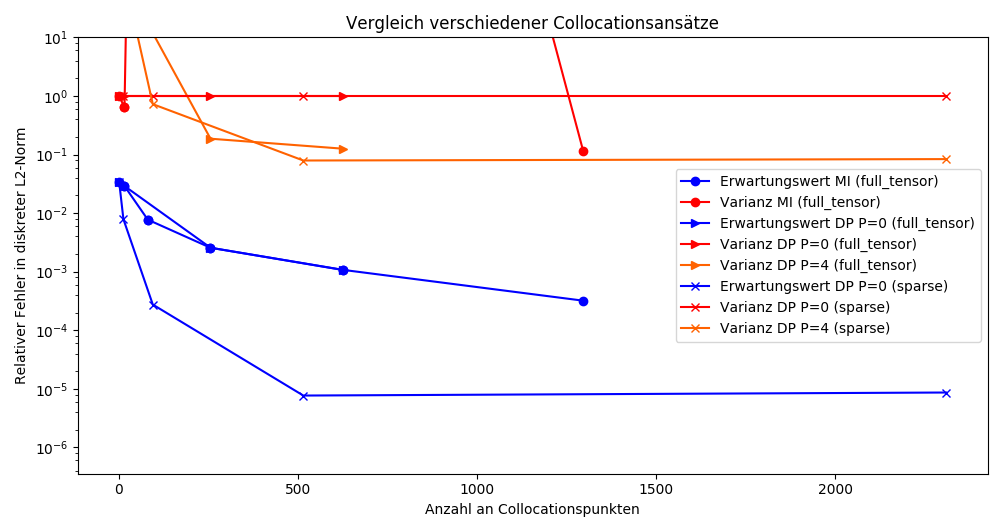
\includegraphics[width=\textwidth]{Figures/collocation_midp_trial8.png}
\caption{Konvergenz der Kollokation für \nameref{trial:8} mit $N=4$ anhand der Anzahl benötigter Kollokationspunkte.}
\label{fig:Kollokation_comparison_trial8}
\end{figure}

\subsubsection*{Unstetige Koeffizienten im Eindimensionalen}
Anhand von \nameref{trial:disconttriple} untersuchen wir die Ansätze für Probleme mit in $y$ unstetigen Koeffizienten $\alpha$ und $\beta$. Dabei ist für $y\in[-1,1]$
\begin{align*}
\alpha(y)&=\begin{cases}2,\quad y>0\\ 1, \quad y\le 0\end{cases}\\
\beta(x,y)&=\begin{cases}2+\sin(x+y),\quad y>0\\ 2+\cos(x+y),\quad y\le 0\end{cases}\\
\end{align*}
Wir erkennen in Abbildung \ref{fig:Kollokation_comparison_trialdiscontsimple} ein unterschiedliches Verhalten für eine gerade bzw. ungerade Anzahl an Quadraturpunkten, die im Eindimensionalen einer gerade bzw. ungerade Anzahl an Basispolynomen entsprechen. Für eine gerade Anzahl an Polynomen konvergieren Erwartungswert und Varianz vergleichbar mit bisherigen Beispielen.
\begin{figure}[!htb]
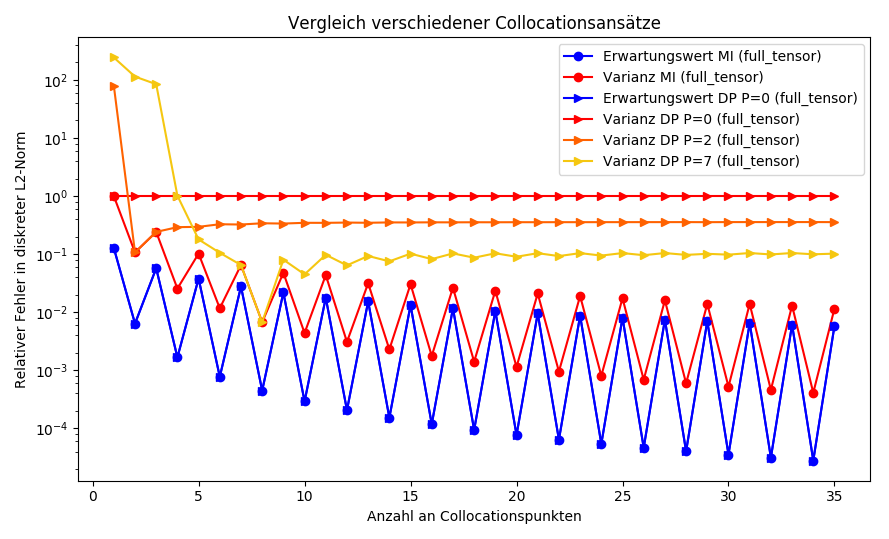
\includegraphics[width=\textwidth]{Figures/collocation_midp_trialdiscontsimple.png}
\caption{Konvergenz der Kollokation für \nameref{trial:discontsimple} mit $N=1$ anhand der Anzahl benötigter Kollokationspunkte.}
\label{fig:Kollokation_comparison_trialdiscontsimple}
\end{figure}
Fügen wir in  eine weitere Unstetigkeitsstelle für $\alpha$ hinzu und entfernen die Unstetigkeit für $\beta$, so ist in Abbildung \ref{fig:Kollokation_comparison_trialdisconttriple} nur noch mit großer Mühe ein Konvergenzverhalten zu erkennen.
\begin{figure}[!htb]
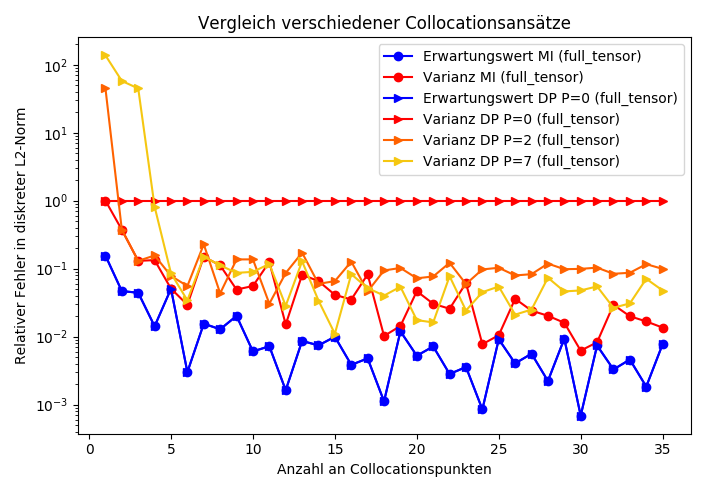
\includegraphics[width=\textwidth]{Figures/collocation_midp_trialdisconttriple.png}
\caption{Konvergenz der Kollokation für \nameref{trial:disconttriple} mit $N=1$ anhand der Anzahl benötigter Kollokationspunkte.}
\label{fig:Kollokation_comparison_trialdisconttriple}
\end{figure}
Für solche Probleme bieten sich adaptive Quadratur- und Interpolationsverfahren an, welche den Träger an bekannten oder unbekannten (Unstetigkeits-) Stellen aufteilen. Dafür ist es hilfreich, die Theorie des gPC auf stückweise Polynome zu erweitern und entsprechende Quadraturverfahren zu verwenden.

 
% Chapter 5

\chapter{Stochastische Galerkin-Methode}
Die stochastische Klein-Gordon-Gleichung war für eine $N$-dimensionale Zufallsvariable $Y$ und $y\in\R^N$ definiert durch
\begin{align}
\label{eqn:galerkin_skgg}
\dtt{u}(t,x,y)&=\alpha(y) \Laplace u(t,x,y) - \beta(x,\omega)u(t,x,y), \: t>0, \, x\in \Torus^d\\
u(0,x,y)&=g(x,y), \: x\in \Torus^d\nonumber\\
\dt{u}(0,x,y)&=h(x,y), \: x\in \Torus^d\nonumber
\end{align}
Seien $\Phi_m(Y)$ die zu $Y$ gehörenden gPC Basisfunktionen. Diese erfüllen die Orthogonalitätsbedingung 
\[\E[\Phi_i(Y)\Phi_j(Y)]=\delta_{ij}\] 
Sei $\Poly_P^N$ der Raum aller Polynome mit summiertem Grad kleiner gleich $P$ und Dimension $\binom{N+P}{P}$. Die gPC Projektion der Lösung der sKGG zu einem fixen Zeitpunkt $T>0$ und Ort $x\in\Torus^d$ ist definiert durch
\begin{align*}
u_M(T,x,Y)&=\sum_{m=0}^M\hat{u}_m(T,x)\Phi_m(Y)\in\Poly_P^N,\quad  M+1=\binom{N+P}{P}\\
\hat{u}_m(T,x)&=\E[u(T,x,Y)\Phi_m(Y)]
\end{align*}
Ist $\rho$ die Dichtefunktion von $Y$, so stimmt die gPC Projektion mit der Bestapproximation in $L_\rho^2$ überein. Diese Approximation ist im $L_\rho^2$ Sinne optimal, allerdings benötigen wir zur Berechnung der Koeffizienten $\hat{u}_m$ die unbekannte exakte Lösung $u(T,x,Y)$.\\
Der stochastische Galerkin Ansatz ist eine Erweiterung des klassischen Galerkin Ansatzes. Sei dazu eine weitere Approximation $v_M\in\Poly_P^N$ gegeben durch
\begin{equation}
v_M(t,x,Y)=\sum_{m=0}^M\hat{v}_m(t,x)\Phi_m(Y)
\end{equation}
Die Forderung an $v_M$ ist dann, dass das Residuum der sKGG (\ref{eqn:galerkin_skgg}) orthogonal zu allen Polynomen aus $\Poly_P^N$ ist. Eine Motivation dafür ist die schwache Lösung der sKGG, welche diese Orthogonalität für alle Polynome $\Poly^N$ erfüllt. Ist die schwache Lösung hinreichend regulär, so stimmt sie mit der Lösung der sKGG überein.
Konkret lautet die Orthogonalitätsbedingung an das Residuum für $t>0$ und $x\in\Torus^d$
\begin{equation}
\label{eqn:galerkinOrtho}
\E\left[\left(\dtt{v_M}(t,x,Y)-\alpha(Y)\Laplace v_M(t,x,Y)+\beta(x,Y)v_M(t,x,Y)\right)\Phi_k\right]=0
\end{equation} 
für alle $k=0,\dots,M$.\\
Wir wollen jetzt aus der Orthogonalitätsbedingung (\ref{eqn:galerkinOrtho}) eine Gleichung für die Koeffizienten $\hat{v}_m$ gewinnen. Dazu setzen wir die Definition von $v_M$ in die Gleichung ein und erhalten
\begin{align*}
\sum_{m=0}^M\dtt{\hat{v}}_m(t,x)\underbrace{\E[\Phi_m(Y)\Phi_k(Y)]}_{=\delta_{mk}}&=\E\left[\alpha(Y)\sum_{m=0}^M\Laplace \hat{v}_m(t,x)\Phi_m(Y)\Phi_k(Y)\right]\\
&\quad -\E\left[\beta(x,Y)\sum_{m=0}^M\hat{v}_m(t,x)\Phi_m(Y)\Phi_k(Y)\right]\\
\equivalent \qquad \dtt{\hat{v}}_k(t,x)&=\sum_{m=0}^M\Laplace \hat{v}_m(t,x)\underbrace{\E[\alpha(Y)\Phi_m(Y)\Phi_k(Y)]}_{=a_{mk}}\\
&\quad -\sum_{m=0}^M\hat{v}_m(t,x)\underbrace{\E[\beta(x,Y)\Phi_m(Y)\Phi_k(Y)]}_{=b_{mk}(x)}\\
\equivalent \qquad \dtt{\hat{v}}_k(t,x)&=a_k\Laplace \hat{v}(t,x)-b_k(x)\hat{v}(t,x)\\
\intertext{mit $ a_k=(a_{0k},\dots,a_{Mk}),\quad b_k(x)=(b_{0k}(x),\dots,b_{Mk}(x)),\quad \hat{v}(t,x)=(\hat{v}_0(t,x),\dots,\hat{v}_M(t,x))^T$}\\
\equivalent \qquad \dtt{\hat{v}}(t,x)&=A\Laplace \hat{v}(t,x)-B(x)\hat{v}(t,x)
\end{align*}
Die Matrizen $A$ und $B(x)$ werden durch die Zeilenvektoren $a_k$ und $b_k(x)$ gebildet und sind symmetrisch. Die benötigten Koeffizienten der Approximation $v_M$ sind gekoppelt und als Lösung folgender partieller Differentialgleichung zu erhalten
\begin{equation}
\label{eqn:galerkin_dgl}
\begin{split}
\dtt{\hat{v}}(t,x)&=A\Laplace \hat{v}(t,x)-B(x)\hat{v}(t,x)\\
\hat{v}(0,x)&=\hat{g}(x)\\
\dt{\hat{v}}(0,x)&=\hat{h}(x)\\
\end{split}
\end{equation}
Dabei gilt für die Anfangswerte $\hat{v}(0,x)$ und $\dt{\hat{v}}(0,x)$ wegen 
\[v_M(0,x,Y)=\sum_{m=0}^M\hat{v}_m(0,x)\Phi_m(Y)\]
und
\begin{align*}
g(x,y)&\approx v_M(0,x,y)\\
h(x,y)&\approx \dt{v}_M(0,x,y)
\end{align*}
die Darstellung mithilfe der Koeffizienten der Bestapproximation von $g$ und $h$
\begin{align*}
\hat{v}_m(0,x)=\hat{g}_m=\E[g(x,Y)\Phi_m(Y)]\\
\dt{\hat{v}}_m(0,x)=\hat{h}_m=\E[h(x,Y)\Phi_m(Y)]
\end{align*}
\section{Splitting für den Galerkin-Ansatz}
Die partielle Differentialgleichung (\ref{eqn:galerkin_dgl}) ist ein System mit Zeitableitung zweiter Ordnung und vektorwertig mit Größe $M+1$. Um eine numerische Lösung des Systems zu erhalten, bietet sich wieder ein Splitting-Ansatz an. Zuerst wollen wir das System aber so weit wie möglich entkoppeln.
\begin{maththeorem}
\label{th:galerkin_posdef}
Ist $\alpha(y)>c$ für ein $c>0$, so ist die Matrix $A$ aus dem Galerkin-Ansatz positiv definit und besitzt nur positive Eigenwerte $\lambda>c$.\\
Ist $\norm{\alpha}_\infty < \infty$, so gilt $\lambda\le \norm{\alpha}_\infty$.
\end{maththeorem}
\begin{proof}
Sei $z\in\R^{M+1}\setminus \lbrace 0\rbrace$ beliebig. Dann gilt wegen $a_{ij}=\int \alpha(y)\Phi_i(y)\Phi_j(y)\rho(y)dy$
\[(Az)_i=\int \alpha(y)\Phi_i(y)\underbrace{\left(\sum_{j=0}^M\Phi_j(y)z_j\right)}_{=\tilde{z}(y)}\rho(y)dy\]
und daher
\begin{align*}
z^TAz&=\int \alpha(y)\left(\sum_{i=0}^M\Phi_i(y)z_i\right)\tilde{z}(y)\rho(y)dy\\
&=\int\underbrace{\alpha(y)}_{>c}\underbrace{\tilde{z}^2(y)}_{>0 \text{ f.ü.}}\underbrace{\rho(y)}_{>0}dy\\
&>c\int \tilde{z}^2(y)\rho(y)dy\\
&=c\sum_{i=0}^Mz_i\sum_{j=0}^Mz_j\underbrace{\int \Phi_i(y)\Phi_j(y)\rho(y)dy}_{=\delta_{ij}}\\
&=cz^Tz
\end{align*}
Die Abschätzung nach oben ergibt sich ähnlich, da für einen Eigenvektor $z\neq 0$ zum Eigenwert $\lambda$ gilt
\[|\lambda| z^Tz=|z^TAz|=\left|\int \alpha(y)\tilde{z}^2(y)\rho(y)dy\right|\leq \norm{\alpha}_\infty z^Tz\]
\end{proof}
Unter entsprechenden Voraussetzungen an $B(x)$ gelten die Aussagen von Satz \ref{th:galerkin_posdef} punktweise auch für $B(x)$.
\subsection{Entkopplung des ersten Teils}
Wir können $A\in\R^{M+1\times M+1}$ zerlegen in
\[A=S_1D_1S_1^T,\quad \text{$D_1$ diagonal und $S_1$ orthogonal}\]
Wir definieren dann 
\[w(t,x)\coloneqq S_1^T\hat{v}(t,x),\quad t>0,x\in\Torus^d\]
und schreiben das System (\ref{eqn:galerkin_dgl}) in der Form
\begin{equation}
\label{eqn:galerkin_dgl_transformed}
\begin{split}
\dtt{w}(t,x)&=D_1\Laplace w(t,x)-S_1^TB(x)S_1w(t,x)\\
w(0,x)&=S_1^T\hat{g}(x)\\
\dt{w}(0,x)&=S_1^T\hat{h}(x)\\
\end{split}
\end{equation}
Schreiben wir es anschließend formal um in ein System mit Zeitableitung erster Ordnung, so gilt für $\tilde{w}\coloneqq \dt w$ und ein Gewicht $\kappa\in[0,1]$
\[\dt\begin{pmatrix}w\\ \tilde{w}\end{pmatrix}(t,x)=\left[\begin{pmatrix}0 & \kappa I_{M+1}\\ D_1\Laplace& 0\end{pmatrix}+\begin{pmatrix}0&(1-\kappa)I_{M+1}\\-S_1^TB(x)S_1 & 0\end{pmatrix}\right]
\begin{pmatrix}w\\\tilde{w}\end{pmatrix}(t,x)\]
Das Splitting besteht dann aus den zwei Gleichungen
\begin{equation}
\label{eqn:galerkin_split1}
\dt\begin{pmatrix}w_1\\ \tilde{w}_1\end{pmatrix}(t,x)=\begin{pmatrix}0 & \kappa I_{M+1}\\ D_1\Laplace& 0\end{pmatrix}\begin{pmatrix}w_1\\\tilde{w}_1\end{pmatrix}(t,x)
\end{equation}
und
\begin{equation}
\label{eqn:galerkin_split2}
\dt\begin{pmatrix}w_2\\ \tilde{w}_2\end{pmatrix}(t,x)=\begin{pmatrix}0&(1-\kappa)I_{M+1}\\-S_1^TB(x)S_1 & 0\end{pmatrix}\begin{pmatrix}w_2\\\tilde{w}_2\end{pmatrix}(t,x)
\end{equation}
Diese sind wie schon in Kapitel \ref{chapter:solver_kgg} mithilfe der Matrixexponentialfunktion lösbar. Beachte, dass die Gleichung (\ref{eqn:galerkin_split1}) nach Umsortierung in $2\times 2$ Systeme entkoppelt ist, da $D_1$ diagonal ist. Die Matrixexponentialfunktion der entkoppelten $2\times 2$ Systeme ist in Algorithmus \ref{alg:kgg_solver} als \emph{First\_Part\_Solver} in einfacher Darstellung direkt gegeben. Der erste Teil des Splittings besteht somit aus dem Lösen von $M+1$ unabhängigen "'Wellengleichungen"' (Name passend für $\kappa=1$). Die Eigenwerte $d_i$ von $A$ sind die Quadrate der Wellengeschwindigkeiten. Abschätzungen für diese, insbesondere Positivität, erhalten wir mithilfe von Satz \ref{th:galerkin_posdef} unter entsprechenden Voraussetzungen an $\alpha(y)$.

\subsection{Entkopplung des zweiten Teils}
Analog zum ersten Teil können wir für jedes fixe $x\in\Torus^d$ die symmetrische Matrix $S_1^TB(x)S_1\in\R^{M+1\times M+1}$ zerlegen in $S_1^TB(x)S_1=S_2(x)D_2(x)S_2^T(x)$ mit $S_2(x)$ orthonormal und $D_2(x)$ diagonal.\\
Definiere
\[z(t,x)\coloneqq S_2^T(x) w_2(t,x), \quad \tilde{z}(t,x)=\dt{z}(t,x)\]
Dann ist (\ref{eqn:galerkin_split2}) äquivalent zum System
\begin{equation}
\label{eqn:galerkin_split2_decoup}
\dt\begin{pmatrix}z\\ \tilde{z}\end{pmatrix}(t,x)=\begin{pmatrix}0&(1-\kappa)I_{M+1}\\-D_2(x) & 0\end{pmatrix}\begin{pmatrix}z\\\tilde{z}\end{pmatrix}(t,x)
\end{equation}
Das System (\ref{eqn:galerkin_split2_decoup}) ist nach Umsortierung in $2\times 2$ Blöcke entkoppelt. Die Matrixexponentialfunktion dieser Blöcke können wir mit der Funktion \emph{Second\_Part\_Solver} aus Algorithmus \ref{alg:kgg_solver} effizient lösen. Der große Vorteil hierbei ist, dass die Berechnung der Matrixexponentialfunktion der $2M+2\times 2M+2$ Matrix aus (\ref{eqn:galerkin_split2}) für jedes $x$ im Gitter entfällt. Der Trade-off ist, dass in jedem Splittingschritt die Transformation und Rücktransformation mit $S_2(x)$ durchgeführt werden muss. Dieser zusätzliche Aufwand fällt jedoch im Gegensatz zur teuren Matrixexponentialfunktion, welche die Blockstruktur der Matrix nicht berücksichtigt, nicht stark ins Gewicht.
\subsection{Algorithmus}
In Algorithmus \ref{alg:galerkin} ist die Vorgehensweise für den Galerkin-Ansatz zum Lösen der stochastischen KGG skizziert. Als Basis dienen dabei die Kernfunktionen des allgemeinen KGG Lösers aus Algorithmus \ref{alg:kgg_solver}, welche in einem schnellen Strang-Splitting eingebettet sind.
\begin{algorithm}[ht]
    \caption{Galerkin für die stochastische KGG.}
    \label{alg:galerkin}
    \begin{algorithmic}[1] % The number tells where the line numbering should start
        \Function{Galerkin}{$H, u_0, v_0, \alpha,\beta,\kappa,Y, M,\tau, T$} 
            	\State $\Phi_m\gets$ $m$-te orthonormale gPC-Basis-Funktion zu $Y$, $\quad m=0,\dots,M$
              \State $A_{mk}\gets \E[\alpha(Y)\Phi_m(Y)\Phi_k(Y)],\quad m,k=0,\dots,M$
              \State $A=S_1D_1S_1^T, \quad S_1$ orthonormal, $D_1$ diagonal
              \State $x_H\gets$ Ortsdiskretisierung der Größe $H$
              \For{$x\in x_H$}
              	\State $B_{mk}(x)\gets \E[\beta(x,Y)\Phi_m(Y)\Phi_k(Y)],\quad m,k=0,\dots,M$
              	\State $S_1^TB(x)S_1=S_2(x)D_2(x)S_2^T(x)$, $S_2(x)$ orthonormal, $D_2(x)$ diagonal
              \EndFor
              \State
              \LineComment{FastStrang Splitting für entkoppelte Systeme:}
              \State $g\gets S_1^T\cdot (\E[u_0(x_H,Y)\Phi_m(Y)])_{m=0,\dots,M}$
              \State $h\gets S_1^T\cdot (\E[v_0(x_H,Y)\Phi_m(Y)])_{m=0,\dots,M}$
              \State $g,h\gets \text{Multi\_First\_Part\_Solver}(H, g, h, \diag(D_1), \kappa, \frac{\tau}{2})$
            \State $g,h\gets \text{Multi\_Second\_Part\_Solver}(x_H, g, h, \diag(D_2), S_2, 1-\kappa, \tau)$
            \For{$i=1,\dots,\frac{T}{\tau}-1$} \Comment{Annahme: $\frac{T}{\tau}\in\N$} 
            	\State $g,h\gets \text{Multi\_First\_Part\_Solver}(H, g, h, \diag(D_1), \kappa, \tau)$
            \State $g,h\gets \text{Multi\_Second\_Part\_Solver}(x_H, g, h, \diag(D_2), S_2, 1-\kappa, \tau)$
            \EndFor
            \State $g,h\gets \text{Multi\_First\_Part\_Solver}(H, g, h, \diag(D_1), \kappa, \frac{\tau}{2})$
            \State
            \LineComment{Rücktransformation und Extraktion der Statistiken:}
            \State $\hat{v}\gets S_1g$  
            \State $\mu\gets \hat{v}_{0,j=1,\dots,H}$ 
			\State $\sigma^2_j\gets \sum_{m=1,\dots,M}\hat{v}^2_{mj}$
			\State \textbf{return} $\mu,\sigma^2$
        \EndFunction
        \Function{Multi\_First\_Part\_Solver}{$H, g, h, \alpha, \kappa, \tau$}
        	\For{$i=0,\dots,M$}
        		\State $\tilde{g}_i,\tilde{h}_i\gets \text{First\_Part\_Solver}(H,g_i, h_i,\alpha_i,\kappa,\tau)$
        	\EndFor
        	\State \textbf{return} $(\tilde{g}_0,\dots,\tilde{g}_M)^T, (\tilde{h}_0,\dots,\tilde{h}_M)^T$
        \EndFunction
        \Function{Multi\_Second\_Part\_Solver}{$x_H,g,h,\beta,S_2,\tilde{\kappa},\tau$}
        	\State $g,h\gets S_2^T(x_H)g, S_2^T(x_H)h$
        	\For{$i=0,\dots,M$}
        		\State $\tilde{g}_i,\tilde{h}_i\gets \text{Second\_Part\_Solver}(x_H,g_i,h_i,\beta_i,\tilde{\kappa},\tau)$
        	\EndFor
        	\State \textbf{return} $S_2(x_H)\cdot (\tilde{g}_0,\dots,\tilde{g}_M)^T, S_2(x_H)\cdot (\tilde{h}_0,\dots,\tilde{h}_M)^T$
        \EndFunction
        
    \end{algorithmic}
\end{algorithm}
Beachte, dass die auftretenden Erwartungswerte zur Berechnung von $A$ und $B(x)$ numerisch mithilfe von Quadraturformeln gelöst werden können. Mögliche Varianten wurden --insbesondere auch für mehrdimensionale Quadratur-- in Kapitel \ref{sec:discrete_proj} vorgestellt. Wir werden die Gauss-Quadratur verwenden, da diese eine hohe polynomiale Exaktheit besitzt und die Wahrscheinlichkeitsdichten implizit berücksichtigt.
\section{Numerische Ergebnisse}
\todo[inline]{Numerische Ergebnisse (über Stopzeit, pro Knotenpunkt,...}
\begin{maththeorem}[Adaption von Theorem 2.2 aus \autocite{davidgottliebdongbinxiu2008}]
\label{th:adapted22}
Ziel: Abschätzung für 
\begin{align*}
\E\left[\norm{u-v_M}_2^2\right]&=\E\left[\int_{-\pi}^{\pi}\left(u(t,x,Y)-v_M(t,x,Y)\right)^2dx\right]\\
&=\int_{-\pi}^\pi\norm{u(t,x,y)-v_M(t,x,y)}_{L_\rho^2}^2dx\\
&\stackrel{\text{Parseval}}{=}\int_{-\pi}^\pi\sum_{m=0}^\infty |\langle u(t,x,y)-v_M(t,x,y),\Phi_m(y)\rangle_{L_\rho^2}|^2dx\\
&=\int_{-\pi}^\pi\sum_{m=0}^\infty\left(\hat{u}_m(t,x)-\hat{v}_m(t,x)\right)^2dx,\quad \hat{v}_m=0 \text{ für } m>M\\
&=\sum_{m=0}^\infty\norm{\hat{u}_m-\hat{v}_m}_2^2\\
&\le \sum_{m=0}^M\norm{\hat{u}_m-\hat{v}_m}_2^2 + \sum_{m=M+1}^\infty \frac{K}{m^{2\ell}}
\end{align*}
\todo[inline]{Problem1: In Vorlage geht Summe nur bis $M$, nicht unendlich.}
\todo[inline]{Problem2: In Vorlage gibt es Voraussetzung 
\[\norm{\hat{u}_m}_2^2\le \norm{\hat{u}_m}_1^2=\int_{-\pi}^\pi\left(\hat{u}^2_m+\left(\dx{\hat{u}_m}\right)^2\right)dx\le \frac{K}{m^{2\ell}},\quad K,\ell>0, m \text{ groß}.\]
Zusammen mit der Summe bis unendlich würde dies einen weiteren Term $\sum_{m=M+1}^\infty \frac{K}{m^{2\ell}}$ auf der rechten Seite der Gesamtabschätzung ergeben. Für $\ell\le\onehalf$ wäre diese Reihe nicht mal konvergent. Wie kommt es, dass dieser Term beim Autor nicht auftaucht?}
\end{maththeorem}
\begin{proof}[Beweisideen]
Sei 
\[e_m(t,x)\coloneqq \hat{u}_m(t,x)-\hat{v}_m(t,x),\quad m=0,\dots,M\]
Verwenden wir den Galerkin-Ansatz (\ref{eqn:galerkinOrtho}) für die Reihendarstellung von $u$ anstelle von $v_M$, so erhalten wir analog zum Ergebnis für $v_M$ die Gleichungen
\begin{equation}
\dtt{\hat{u}}_k(t,x)=\sum_{m=0}^\infty \Laplace \hat{u}_m(t,x)a_{mk}-\sum_{m=0}^\infty \hat{u}_m(t,x)b_{mk}(x),\quad k=0,\dots,M
\end{equation}
Subtrahieren wir davon die Gleichungen
\begin{equation}
\dtt{\hat{v}}_k(t,x)=\sum_{m=0}^M\Laplace \hat{v}_m(t,x)a_{mk}-\sum_{m=0}^M\hat{v}_m(t,x)b_{mk}(x),\quad k=0,\dots,M
\end{equation}
so erhalten wir für $k=0,\dots,M$
\begin{equation}
\label{eqn:error_eq_1}
\begin{split}
\dtt{e_k}(t,x)&=\sum_{m=0}^M\Laplace e_m(t,x)a_{mk}-\sum_{m=0}^M e_m(t,x)b_{mk}(x)\\
&\quad +\sum_{m=M+1}^\infty \Laplace \hat{u}_m(t,x)a_{mk}-\hat{u}_m(t,x)b_{mk}(x)
\end{split}
\end{equation}
Nun definieren wir $e\coloneqq (e_0,\dots,e_M)^T, f\coloneqq S_1^Te$ und schreiben Gleichung (\ref{eqn:error_eq_1}) kompakt als
\begin{equation}
\label{eqn:error_eq2}
\dtt{f}=D_1\Laplace f-S_1^TB(x)S_1f+r
\end{equation}
Dabei ist $S_1D_1S_1^T=A$ und $r$ der Restterm der Gleichung mit
\[r_{i}(t,x)=\sum_{k=0}^Ms_{ki}\sum_{m=M+1}^\infty \Laplace \hat{u}_m(t,x)a_{mk}-\hat{u}_m(t,x)b_{mk}(x)\]
Wir multiplizieren Gleichung (\ref{eqn:error_eq2}) nun von links mit $f^T$ und integrieren über $x$
\begin{align*}
\int_{-\pi}^\pi f^T(t,x)\dtt{f}(t,x)dx&=\sum_{i=0}^M d_i\int_{-\pi}^\pi f_i(t,x)\Laplace f_i(t,x)dx\\
&\quad -\int_{-\pi}^\pi f^T(t,x)S_1^TB(x)S_1f(t,x)dx+\int_{-\pi}^\pi f^Trdx
\end{align*}
Ist $\alpha(y)>c>0$, so ist nach Satz \ref{th:galerkin_posdef} auch $d_i>c$. Weiterhin gilt aufgrund der periodischen Randbedingung mit dem Satz von Green
\[\int_{-\pi}^\pi f_i(t,x)\Laplace f_i(t,x)dx=-\int_{-\pi}^\pi \norm{\nabla f_i(t,x)}^2dx+\underbrace{\oint f_i(t,x)(\nabla f_i\cdot n)d\sigma}_{=0}\le 0\]
Daher ergibt sich die Abschätzung
\begin{equation}
\int_{-\pi}^\pi f^T(t,x)\dtt{f}(t,x)dx\le \int_{-\pi}^\pi f^Tr\,dx\le \norm{f}_2\norm{r}_2 
\end{equation}
\todo[inline]{Problem3: Ich finde keine gute Möglichkeit daraus eine Abschätzung für $\norm{f}_2$ zu erhalten. Mithilfe dieser hätte ich dann auch eine Abschätzung für $\norm{e}_2$ und somit für den Satz. Evtl. mit einer anderen Norm als der verwendeten $\norm{g}_2^2\coloneqq \int_{-\pi}^\pi g^2(x)dx$ um die Ableitung nach der Zeit zweiter Ordnung besser in den Griff zu bekommen?}
\end{proof}
Wir beobachten in den Abbildungen \ref{fig:galerkin_bystoptime_trial1_low} und \ref{fig:galerkin_bystoptime_trial1_high} das Verhalten für wachsende Stoppzeit $T$ anhand der einfachen \nameref{trial:1}. Die Parameter für die Quadratur sind dabei hoch genug gewählt um als relevante Fehlerquellen ausgeschlossen werden zu können. 
\todo[inline]{Beobachtungen?!}
\begin{figure}[!htb]
\minipage{0.55\textwidth}
  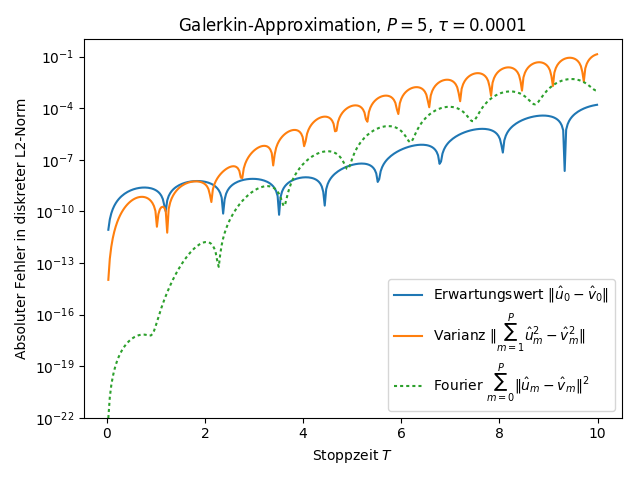
\includegraphics[width=\linewidth]{Figures/galerkin_bystoptime_trial1_fixeddegree5.png}
\endminipage
\minipage{0.55\textwidth}
  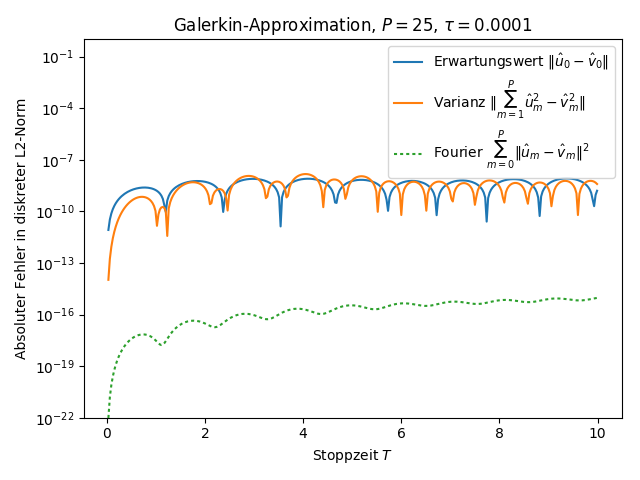
\includegraphics[width=\linewidth]{Figures/galerkin_bystoptime_trial1_fixeddegree25.png}
\endminipage
  \label{fig:galerkin_bystoptime_trial1}
  \caption{Verschiedene Fehler von \nameref{trial:1} mit fixem Polynomgrad und hinreichend guter Quadraturformel.}
\end{figure}
\todo[inline]{Problem4: Es ist nicht ganz klar, was eigentlich rauskommen soll. Durch fehlende Referenzlösungen für die Varianz an vielen verschiedenen Zeitpunkten ist es schwierig, beliebige Beispiele zu beobachten.}
Schlussendlich sehen wir in den Abbildungen \ref{fig:galerkin_bydegree_trial1_t1} und \ref{fig:galerkin_bydegree_trial1_t5} das Verhalten des Fehlers in Abhängigkeit von der Anzahl an Polynomen $P=M+1$. Zum Zeitpunkt $T=1$ wird für $P>5$ der Fehler minimal, für $T=5$ passiert die bestmögliche Approximation allerdings erst für $P>8$. Diese benötigte Grenze wächst mit größerem $T$. 
\begin{figure}[!htb]
\centering
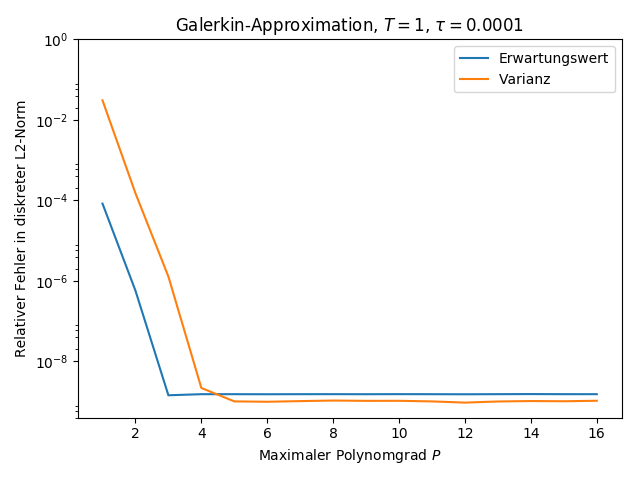
\includegraphics[width=0.5\linewidth]{Figures/galerkin_bydegree_trial1_t1.png}
\caption{Approximation des Erwartungswert und der Varianz von \nameref{trial:1} zu fixem Zeitpunkt $T=1$ durch Galerkin-Ansatz mit $\tau=0.0001$ und verschiedenen Polynomgraden.}
\label{fig:galerkin_bydegree_trial1_t1}
\end{figure}

\begin{figure}[!htb]
\centering
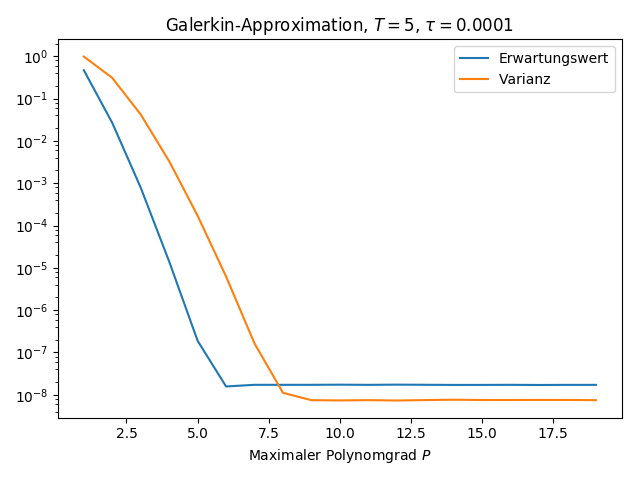
\includegraphics[width=0.5\linewidth]{Figures/galerkin_bydegree_trial1_t5.png}
\caption{Approximation des Erwartungswert und der Varianz von \nameref{trial:1} zu fixem Zeitpunkt $T=5$ durch Galerkin-Ansatz mit $\tau=0.0001$ und verschiedenen Polynomgraden.}
\label{fig:galerkin_bydegree_trial1_t5}
\end{figure}
\subsection{Vergleich Galerkin und Collocation}
\todo[inline]{Vergleiche mehrdim, unstetig, nicht diffbar mit Collocation} 

%----------------------------------------------------------------------------------------
%	THESIS CONTENT - APPENDICES
%----------------------------------------------------------------------------------------

\appendix % Cue to tell LaTeX that the following "chapters" are Appendices

% Include the appendices of the thesis as separate files from the Appendices folder
% Uncomment the lines as you write the Appendices

% Appendix A

\chapter{Orthogonale Polynome im Askey Schema} % Main appendix title

\label{AppendixA} % For referencing this appendix elsewhere, use \ref{AppendixA}

\section{Geschichtliche Entstehung}
Die Entstehung des \emph{general Polynomial Chaos}(gPC) ist eine Geschichte über den Versuch, stochastische Abhängigkeit und Integrationstheorie zu kombinieren. Sie wurzelte in der Arbeit von Wiener (\autocite{norbertwiener1938}), wo er das \emph{homogene Chaos} einführte, um die Entwicklung von Unsicherheit in einem dynamischen, chaotischen, physikalischen System zu konkretisieren. Dies erklärt auch den Ursprung der Bezeichnung "`Chaos"' im Kontext der chaotischen Brownschen Bewegung im Wiener-Prozess.\\
Ghanem verwendete dann Hermite Polynome um mithilfe dieser Orthogonalbasis gaußsche Prozesse darzustellen. Dies wendete er erfolgreich auf einige Probleme aus den Ingenieurswissenschaften an, ein Überblick wird in \autocite{GhaSpa91} gegeben.\\
Xiu verallgemeinerte in seiner Arbeit \autocite{xiu2002} diesen Ansatz auf andere Kombinationen aus stochastischer Verteilung und Polynombasis. Gemäß dem Askey Schema (siehe Abbildung \ref{askeyscheme}) werden Beziehungen einiger bekannter Polynom Orthonormalbasen verdeutlicht. Man beobachtet außerdem, dass einige Gewichte den Dichtefunktionen von bekannten Verteilungen entsprechen und möchte nun zu einer gegebenen Verteilung die bestmögliche Polynombasis verwenden. An Modellproblemen demonstrierte Xiu jeweils optimale exponentielle Konvergenz für die verschiedenen Paarungen.\\
\begin{figure}
\center
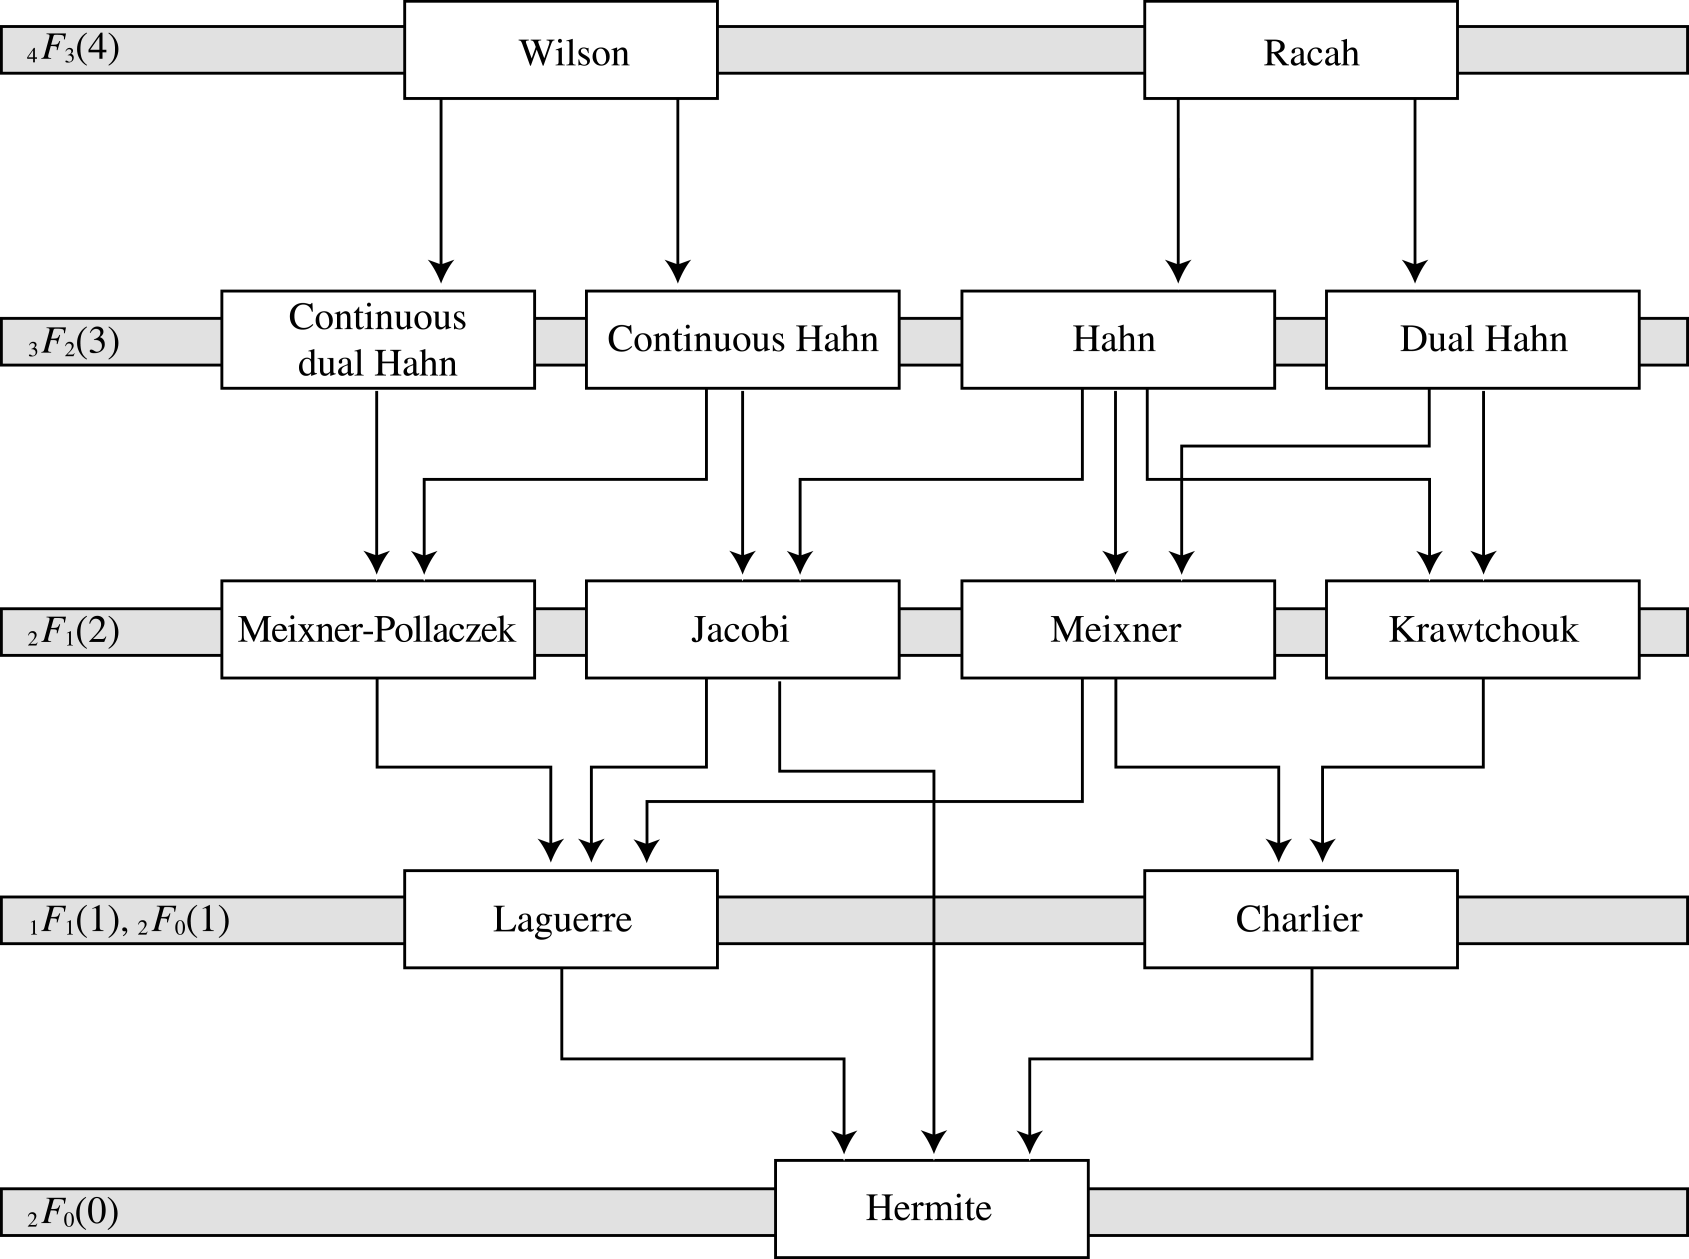
\includegraphics[width=0.8\linewidth]{Figures/askeyscheme.png}
\caption{Askey Schema; Ein Pfeil symbolisiert den Übergang einer Basis in eine andere durch Grenzwertbildung eines Parameters; Quelle: \autocite{webaskey}}
\label{askeyscheme}
\end{figure}
\begin{mathbsp}[Grenzwertbildung im Askey Schema]
Es gilt für die Jacobi Polynome $P_n^{(\alpha,\beta)}(x)$ und die Hermite Polynome $H_n(x)$ die Beziehung
\[\lim\limits_{\alpha\to\infty}\alpha^{-\onehalf n}P_n^{(\alpha,\alpha)}\left(\frac{x}{\sqrt{\alpha}}\right)=\frac{H_n(x)}{2^nn!}\]
Für eine genauere Betrachtung der Beziehungen der hypergeometrischen Polynome im Askey Schema sei auf \autocite{koekoekswart98} verwiesen.
\end{mathbsp}

\section{Auflisting von Polynombasen und Verteilungen}
Wir präsentieren hier eine Auswahl der von uns verwendeten Orthogonalpolynome, insbesondere ihre Definition, Darstellung als Drei Term Rekursion, Gewichtsfunktion und ihre Beziehung zu stochastischen Verteilungen. Für weitere Eigenschaften wie die Darstellung als Lösung einer Differentialgleichung oder die Rodriguez Formel sei beispielsweise auf den Anhang von \autocite{dongbinxiu2010} verwiesen.\\
Eine schöne Übersichtstabelle findet sich unter \url{http://dlmf.nist.gov/18.3}, man beachte, dass dort die verwendeten Polynome und Gewichte teilweise von unserer Notation abweichen. Dies ist der Tatsache geschuldet, dass die Beziehung zu Verteilungen und entsprechende Normierungsanforderungen keine Rolle spielen. Ebenso gibt es verschiedene Varianten die untere Grenze für die Parameter $\alpha$ und $\beta$ der Jacobi und Laguerre Polynome zu definieren.\\
Benötigt man Referenzwerte für Nullstellen und Gewichte einer zugehörigen Gauss Quadratur, so findet sich unter\\\url{http://keisan.casio.com/exec/system/1281279441} ein Onlinerechner. Hierbei sei wieder auf abweichende Notation hingewiesen, insbesondere die fehlende Normierung der Gewichte um einen Faktor.\\
Um die Polynome möglichst kompakt darzustellen zu können, werden folgende Definitionen nützlich sein.
\begin{mathdef}[Pochhammer Symbol]
Das Pochhammer Symbol $(a)_n$ für $a\in\R$ und $n\in\lbrace -1,0,1,2,\dots\rbrace$ sei definiert durch
\[(a)_n=\frac{\Gamma(a+n)}{\Gamma(a)}=
   \begin{cases}
   1, &n=-1\text{ oder } n=0\\
   a(a+1)\dots (a+n-1), &n\in\N
   \end{cases}
   \]
Beachte, dass dies auch \emph{steigende Fakultät} genannt wird und nicht mit der \emph{fallenden Fakultät} verwechselt werden sollte, wie das Symbol auch manchmal verwendet wird. Die Notation ist in der Literatur nicht einheitlich!
\end{mathdef}

\begin{mathdef}[Hypergeometrische Funktion]
Zu $r,s\in\N_0$ ist die hypergeometrische Funktion $_rF_s$ definiert durch
\[_rF_s(a_1,\dots,a_r;b_1,\dots,b_s;z)\coloneqq \sum_{k=0}^\infty \frac{(a_1)_k\dots (a_r)_kz^k}{(b_1)_k\dots(b_s)_kk!}\]
\end{mathdef}
Für weitere Polynome aus dem Askey Schema (siehe Abbildung \ref{askeyscheme}), insbesondere diese mit diskreten Verteilungen, sei wieder beispielsweise auf \autocite{dongbinxiu2010} verwiesen. \\
Für eine Methode zum Berechnen der Nullstellen aus der Drei Term Rekursion steht der Golub Welsch Algorithmus (vgl. \ref{golubwelschalg}) zur Verfügung.\\
Für die Drei-Term-Rekursion der nicht normalisierten orthogonalen Polynome $\Psi_n$ gilt stets $\Psi_{-1}\equiv 0$ und $\Psi_{0}\equiv 1$.
\subsection{Hermite Polynome und Gauß Verteilung}
Träger:
\[I=\R\]
Definition:
\[H_n(x)=(2x)^n\cdot {_2F_0}\left(-\frac{n}{2},-\frac{n-1}{2};\, ;-\frac{2}{x^2}\right)\]
Drei-Term-Rekursion:
\[H_{n}(x)=xH_{n-1}(x)-(n-1)H_{n-2}(x)\]
Gewichtsfunktion:
\[w(x)=\frac{1}{\sqrt{2\pi}}e^{-\frac{x^2}{2}}\]
Normalisierungsfaktor:
\[\gamma_n=n!\]
Stochastische Verteilung:
\begin{center}
normalisierte Gauß Verteilung mit Dichtefunktion $\rho(x)=w(x)$
\end{center}

\subsection{Laguerre Polynome und Gamma Verteilung}
Träger:
\[I=(0,\infty)\]
Definition:
\[L_n^{(\alpha)}(x)=\frac{(\alpha)_n}{n!}\cdot {_1F_0}\left(-n;\alpha;x\right),\quad \alpha>0\]
Drei-Term-Rekursion:
\[L_{n}^{(\alpha)}(x)=\frac{2n-2+\alpha -x}{n}L_{n-1}^{(\alpha)}(x)-\frac{n-1+\alpha - 1}{n}L_{n-2}^{(\alpha)}(x)\]
Gewichtsfunktion:
\[w(x)=\frac{x^{\alpha-1}e^{-x}}{\Gamma(\alpha)}\]
Normalisierungsfaktor:
\[\gamma_n=\frac{(\alpha)_n}{n!}\]
Stochastische Verteilung:
\begin{center}
Gamma Verteilung mit $\alpha>0,\beta=1$ und Dichtefunktion
\[\rho(x)=\frac{x^{\alpha-1}e^{-\frac{x}{\beta}}}{\beta^{\alpha}\Gamma(\alpha)}\]
\end{center}

\subsection{Jacobi Polynome und Beta Verteilung}
Träger:
\[I=(-1,1)\]
Definition:
\[P_n^{(\alpha, \beta)}(x)=\frac{(\alpha + 1)_n}{n!}\cdot {_2F_1}\left(-n,n+\alpha+\beta+1;\alpha+1;\frac{1-x}{2}\right),\quad \alpha,\beta>-1\]
Drei-Term-Rekursion:
\begin{center}
Zum Abkürzen sei für $n\in\N\quad f_n \coloneqq \frac{(2n + \alpha + \beta - 1)(2n + \alpha + \beta)}{2n(n + \alpha + \beta)}$
\begin{align*}
P_n^{(\alpha, \beta)}(x)&=\left(f_nx-\frac{f_n(\beta^2-\alpha^2)}{(2n + \alpha + \beta - 2)(2n + \alpha +\beta)}\right)P_{n-1}^{(\alpha, \beta)}(x)\\
&\quad-\frac{2f_n(n + \alpha - 1)(n + \beta - 1)}{(2n + \alpha + \beta - 2)(2n + \alpha + \beta - 1)}P_{n-2}^{(\alpha, \beta)}(x)
\end{align*}
Man beachte, dass dies einige Definitionslücken aufweist:
\begin{itemize}
\item Für $\alpha=\beta=0$ stimmen die Jacobi Polynome exakt mit den Legendre Polynomen überein und die Betaverteilung mit der Gleichverteilung (siehe \ref{seclegendre}).
\item Für $\alpha+\beta=0,n=1$ gilt $P_1^{(\alpha,\beta)}(x)=x-\frac{\beta-\alpha}{2}$
\item Für $\alpha+\beta=-1,n=1$ gilt $P_1^{(\alpha,\beta)}(x)=\frac{x}{2}-\frac{\beta-\alpha}{2}$
\end{itemize}
\end{center}
Gewichtsfunktion:
\[w(x)=\frac{\Gamma(\alpha+\beta+2)}{2^{\alpha+\beta+1}\Gamma(\alpha+1)\Gamma(\beta+1)}(1-x)^\alpha(1+x)^\beta\]
Normalisierungsfaktor:
\[\gamma_n=\frac{(\alpha+1)_n(\beta+1)_n}{n!(2n+\alpha+\beta+1)(\alpha+\beta+2)_{n-1}}\]
Stochastische Verteilung:
\begin{center}
Beta Verteilung auf $(-1,1)$ mit $\alpha,\beta>-1$ und Dichtefunktion
\[\rho(x)=\frac{(1 - x)^\alpha(1 + x)^\beta}{2^{\alpha + \beta + 1}B(\alpha+1,\beta+1)}=w(x),\quad B\text{ ist Eulersche Betafunktion}\]
\end{center}

\subsection{Legendre Polynome und Gleichverteilung}
\label{seclegendre}
Als wichtiger Spezialfall der Jacobi Polynome seien die Legendre Polynome an dieser Stelle explizit erwähnt.\\
Träger:
\[I=[-1,1]\]
Definition:
\[L_n(x)={_2F_1}\left(-n,n+1;1;\frac{1-x}{2}\right)\]
Drei-Term-Rekursion:
\[L_{n}(x)=x\frac{2n-1}{n}L_{n-1}(x)-\frac{n-1}{n}L_{n-2}(x)\]
Gewichtsfunktion:
\[w(x)\equiv \onehalf\]
Normalisierungsfaktor:
\[\gamma_n=\frac{1}{2n+1}\]
Stochastische Verteilung:
\begin{center}
Gleichverteilung auf $[-1,1]$ mit Dichtefunktion $\rho(x)=w(x)$
\end{center}

\include{Appendices/AppendixB}
%\include{Appendices/AppendixC}

%----------------------------------------------------------------------------------------
%	BIBLIOGRAPHY
%----------------------------------------------------------------------------------------
% \nocite{*}  % uncomment if we do not cite everything but want to include full .bib file
\nocite{latextemplate}
\printbibliography[heading=bibintoc]

%----------------------------------------------------------------------------------------

\end{document}  
